\section{The final Weekplanner application}

During the report, we have described the work we have done on the Weekplanner application. After sprint 4 we did not develop the Weekplanner further, so the release of this sprint was the product that will be handed over to next year students. This section describes the visual content and the features of the Weekplanner application, but not the technical aspects of it.

There are eight screens in the Weekplanner application. These are listed below:

\begin{itemize}
    \item Login screen
    \item Choose citizen screen
    \item Week-plan selection screen
    \item New week-plan screen
    \item Week-plan screen
    \item Pictogram search screen
    \item Show activity screen
    \item Upload image from device screen
\end{itemize}

Here follows a description of each of the screens and their functionality.

\subsection{Login Screen}

The login screen does not have other functions than login and is the first screen when opening the application. In \autoref{fig:FinalLoginScreen} we see the final login screen.

\begin{figure}[H]
    \begin{center}
        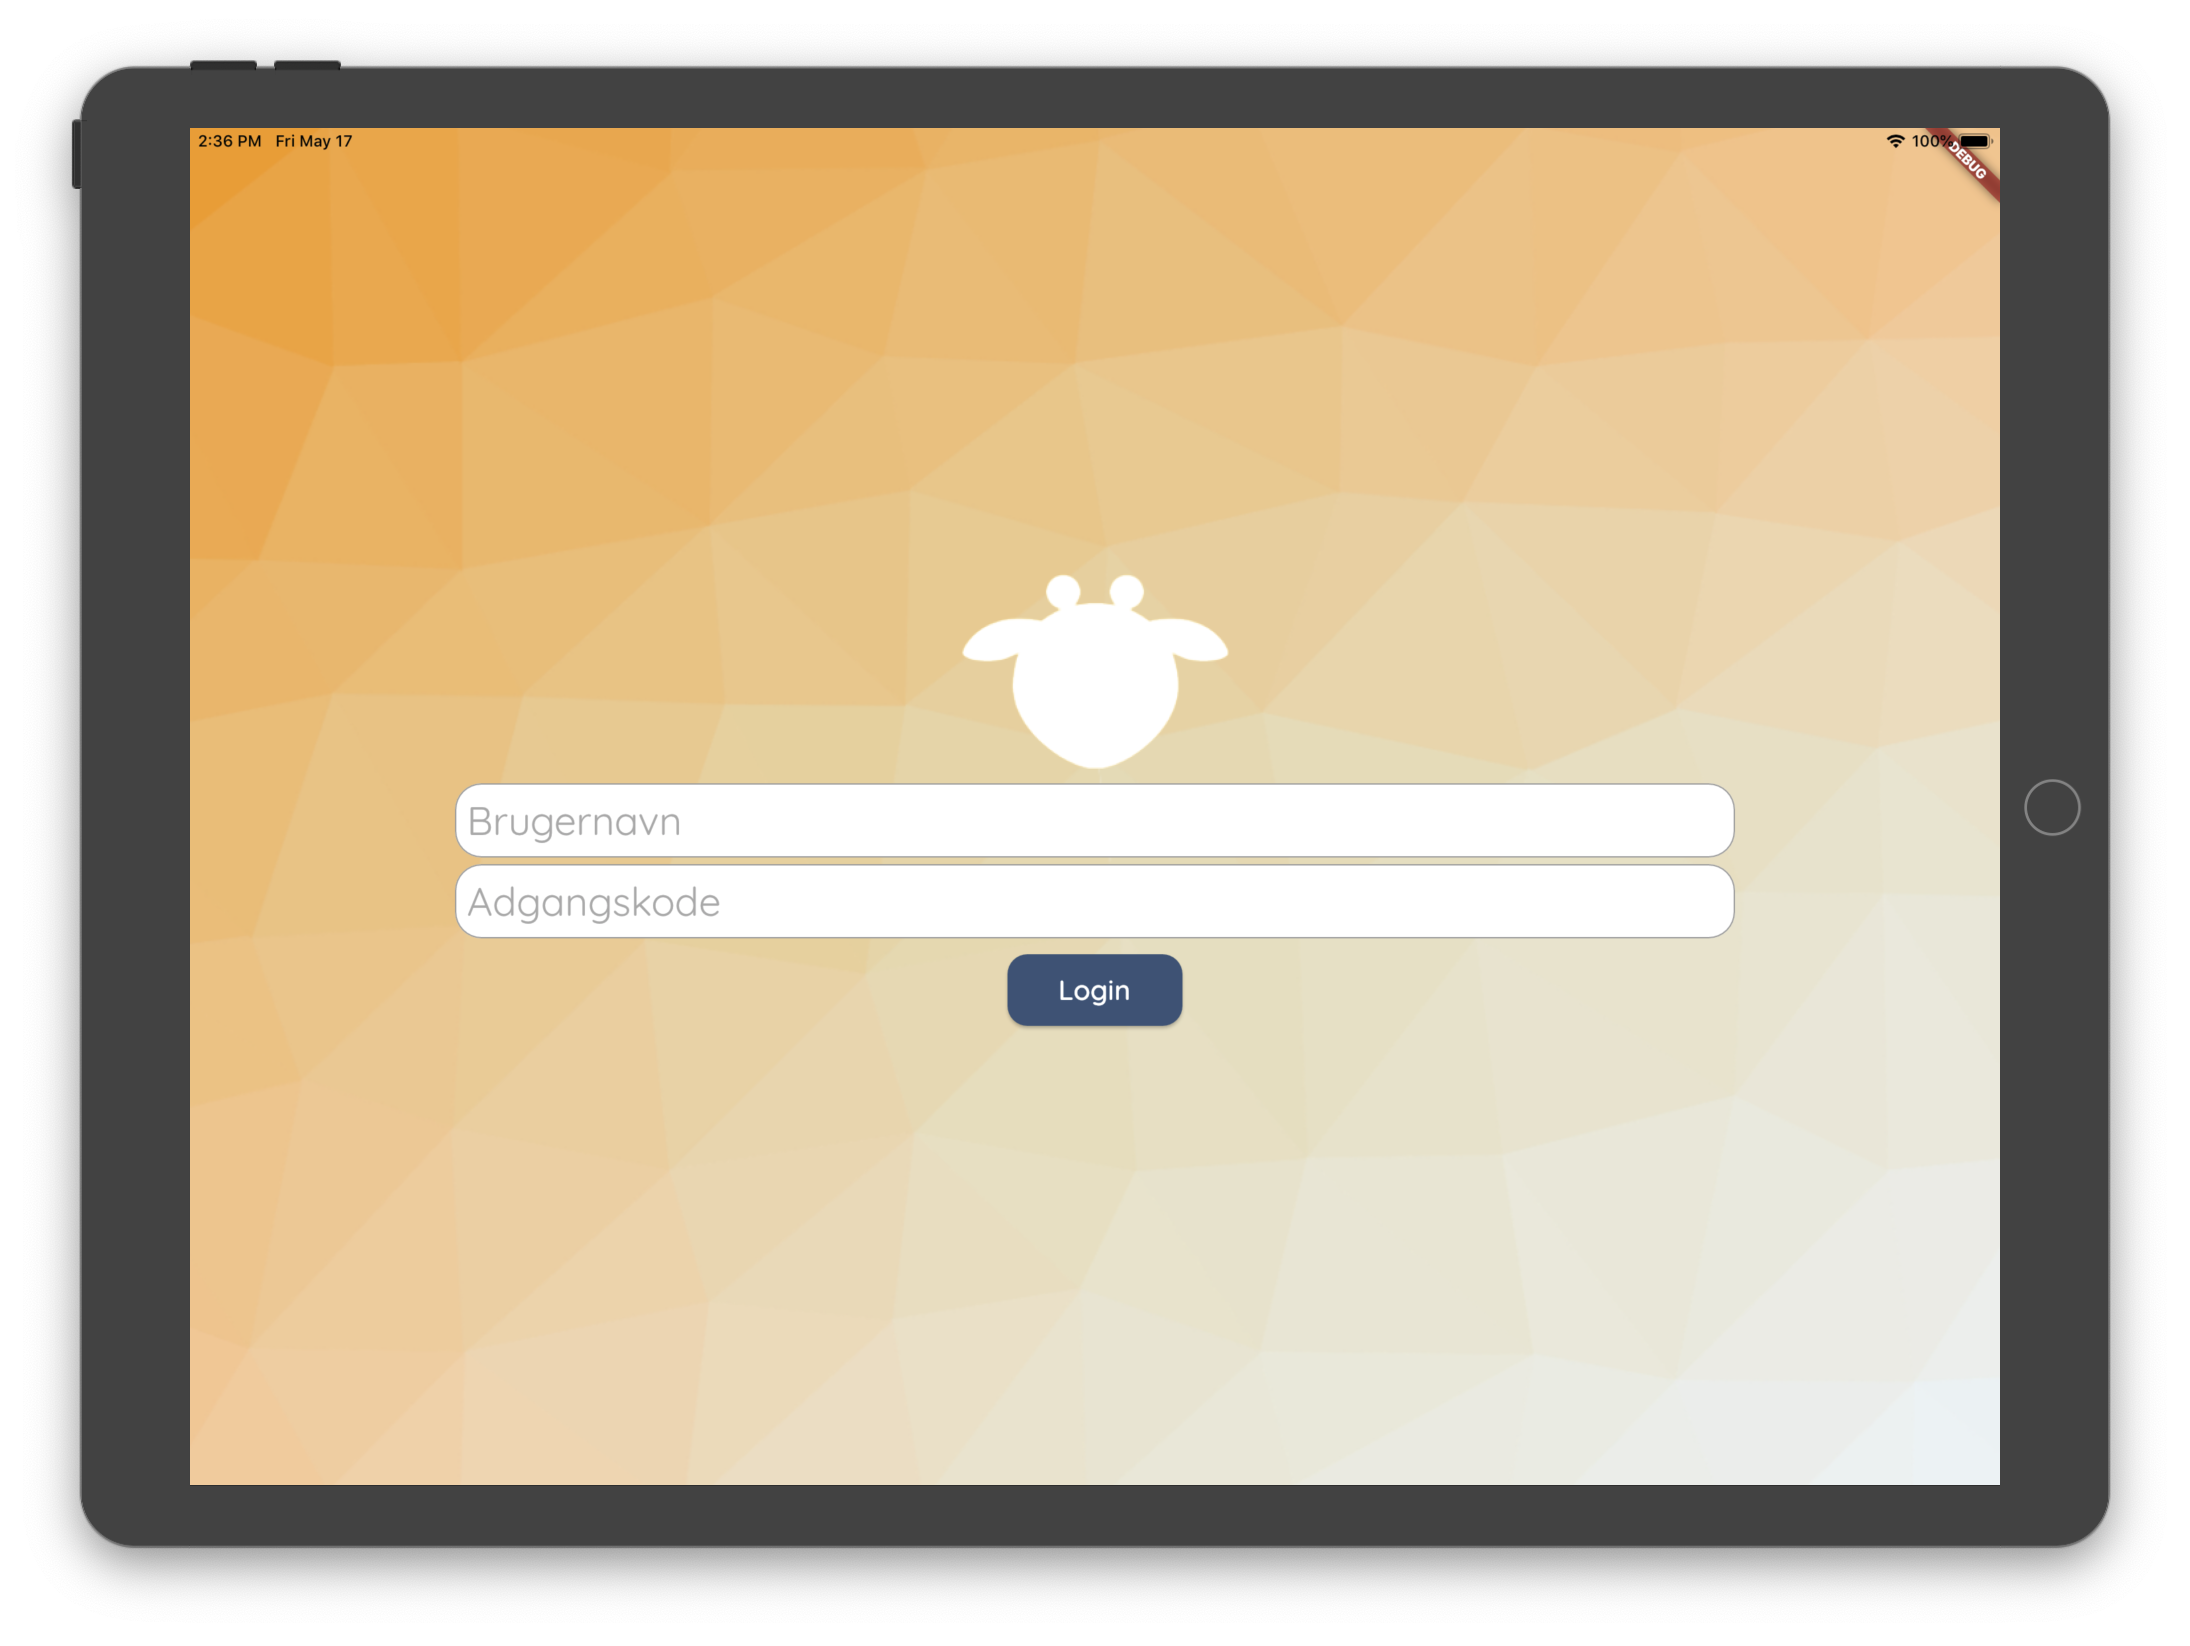
\includegraphics[width=0.7\textwidth]{figures/FinalScreen/loginScreen.png}
    \end{center}
    \caption{The final login screen}
    \label{fig:FinalLoginScreen}
\end{figure}

\subsection{Choose Citizen Screen}

On the citizen screen, we see an overview of the \glspl{citizen} connected to the logged in user, and we can choose a specific \gls{citizen}. The screen shows their names but not their avatars. We can either choose a citizen or log out of the application. \autoref{fig:finalCitizenScreen} shows the final screen.

\begin{figure}[H]
    \begin{center}
        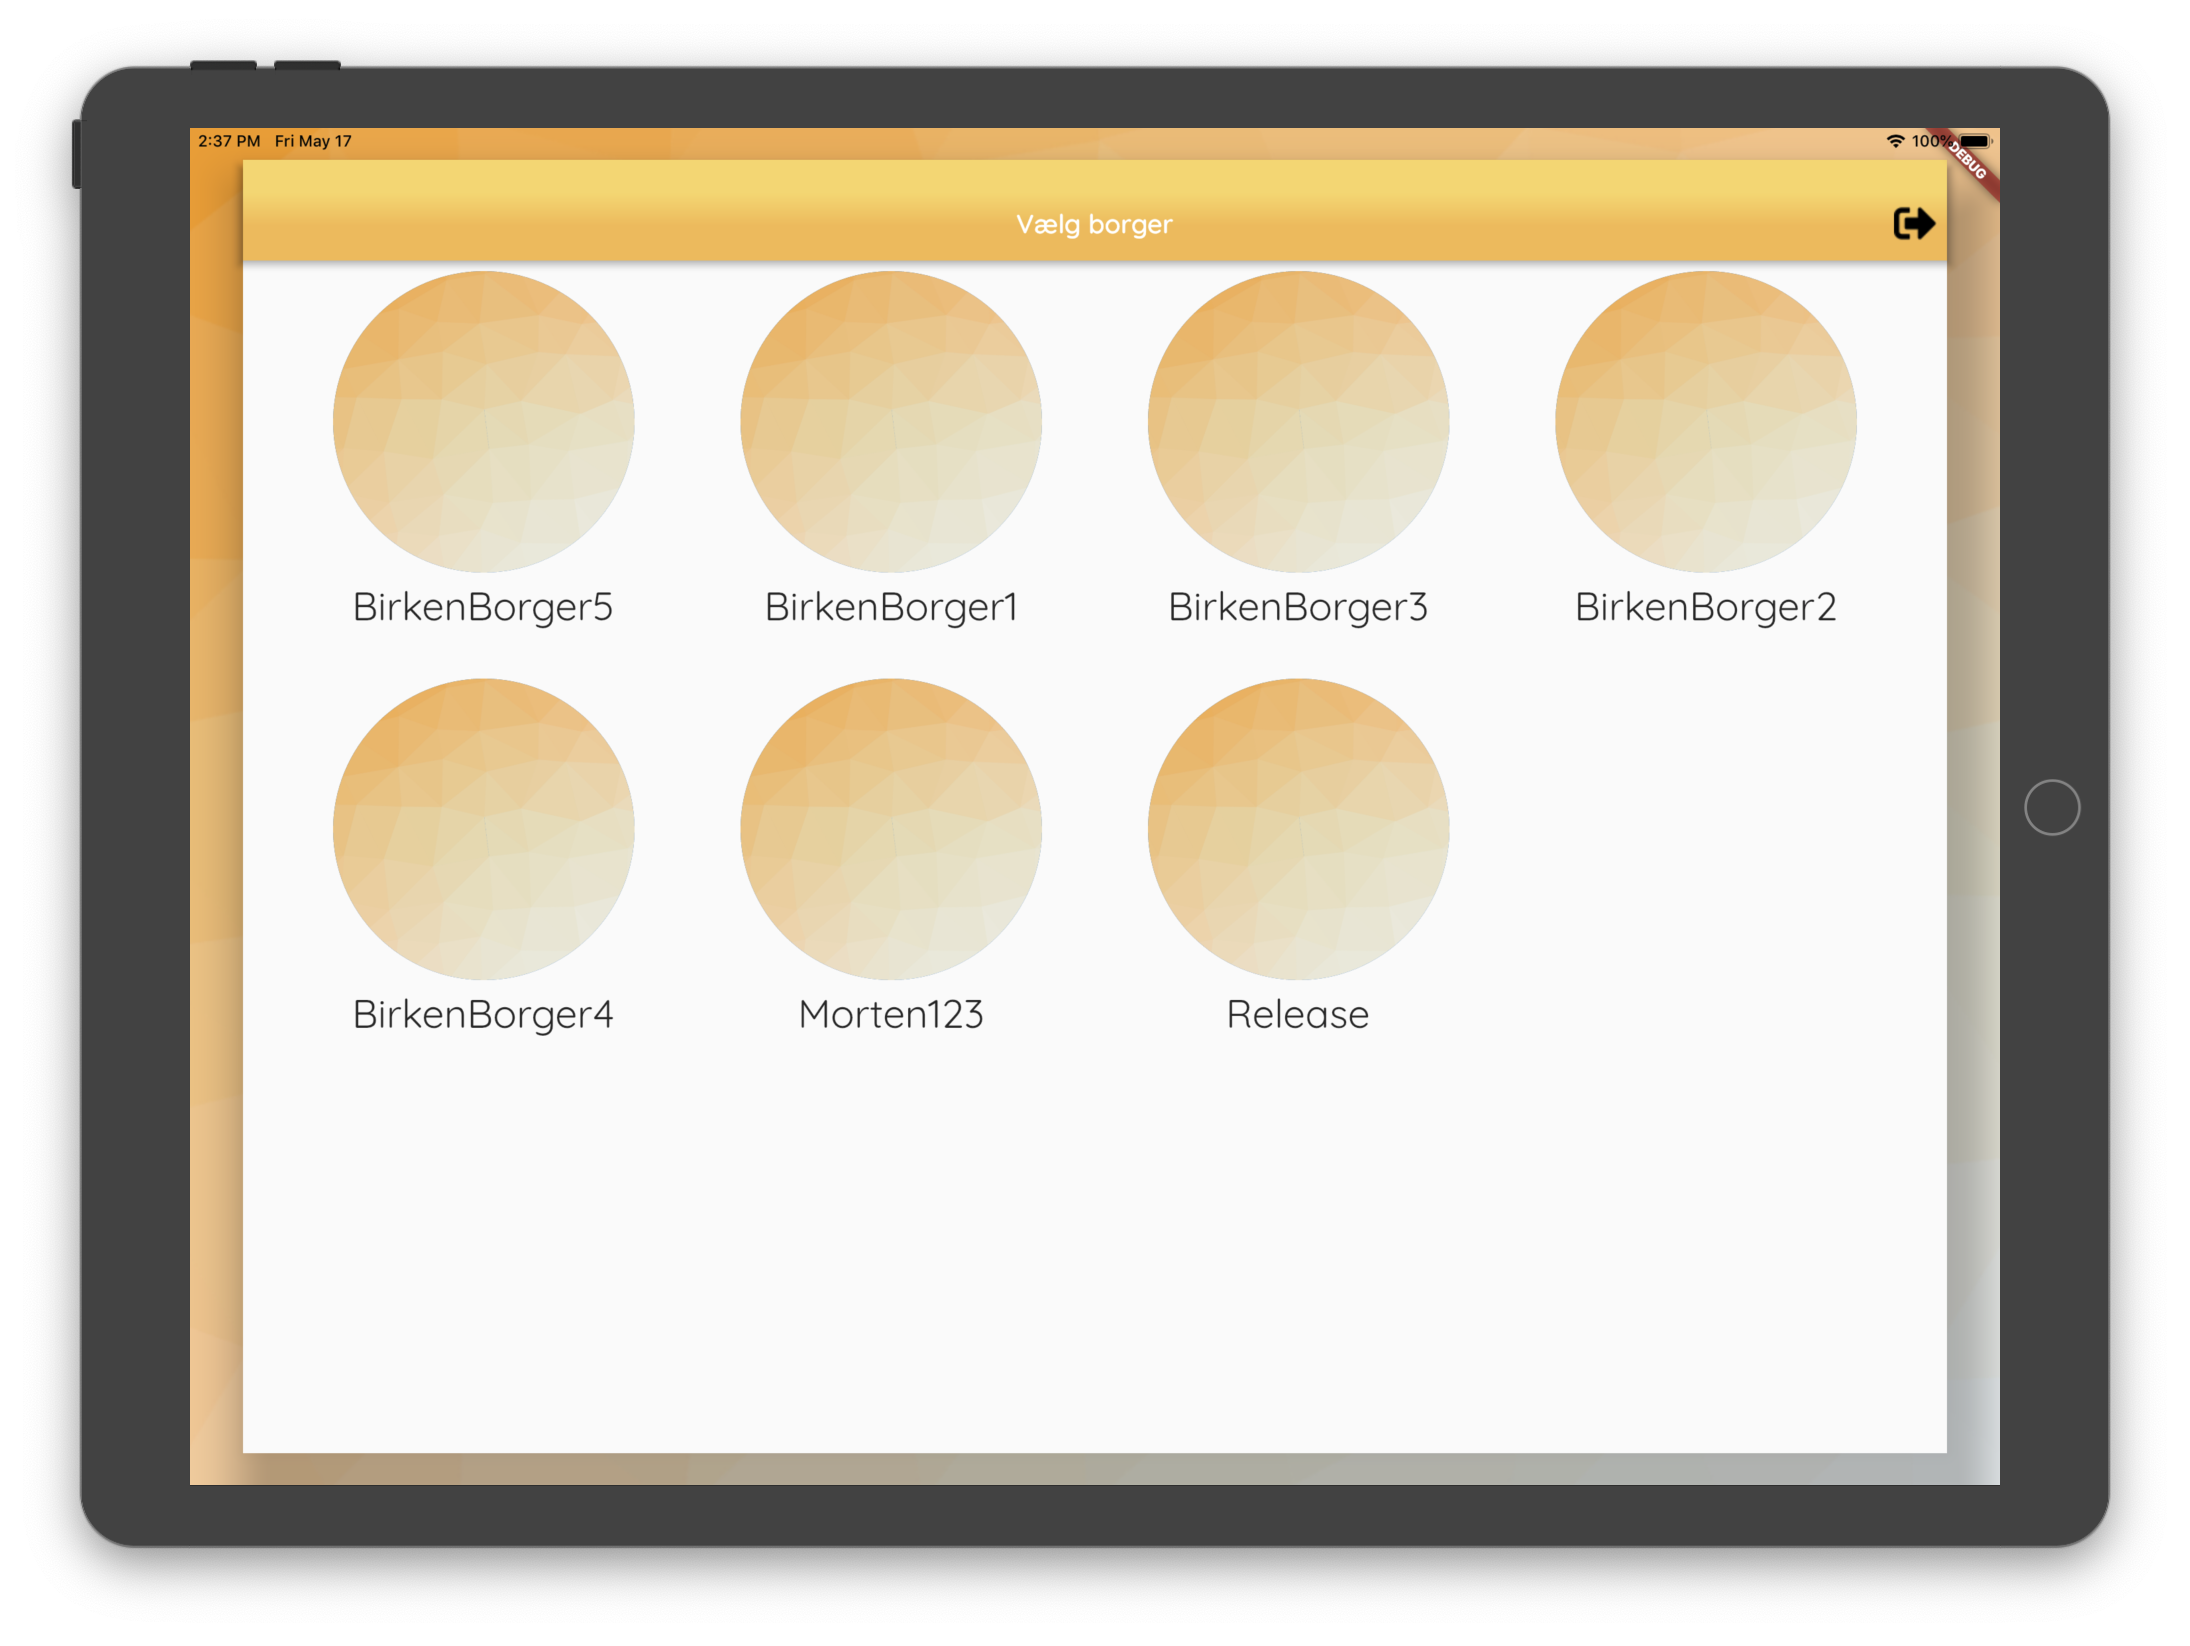
\includegraphics[width=0.7\textwidth]{figures/FinalScreen/chooseCitizenScreen.png}
    \end{center}
    \caption{The final \gls{citizen} screen}
    \label{fig:finalCitizenScreen}
\end{figure}

\subsection{Weekplan selector screen}

The week-plan selector screen has two modes, a selector mode, and a deletion mode, both shown in \autoref{fig:finalEditWeekplanSelector}.

\begin{figure}%
    \centering
    \subfloat[Selection]{{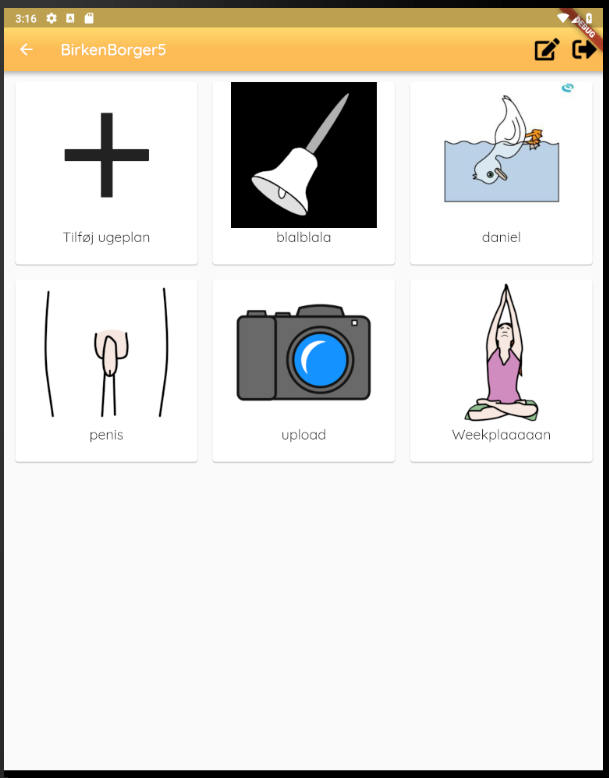
\includegraphics[width=0.45\textwidth]{figures/FinalScreen/chooseWeekplanScreen.png} }}%
    \quad
    \subfloat[Deletion]{{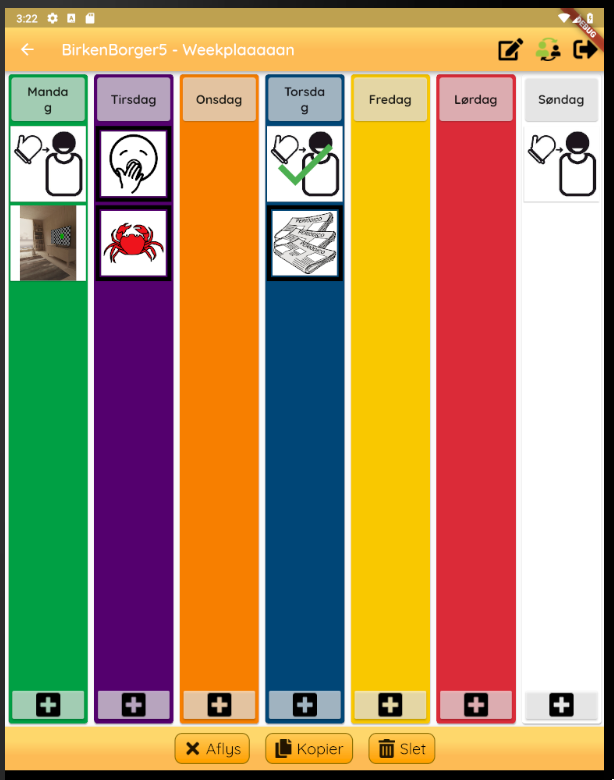
\includegraphics[width=0.45\textwidth]{figures/FinalScreen/editWeekplanScreen.png} }}%
    \caption{The final choose week-plan screen in its two different modes}%
    \label{fig:finalEditWeekplanSelector}%
\end{figure}

In selection mode, we can either create a new week-plan or choose an already existing week-plan. In the deletion mode, we can delete a variable number of week-plans. The week-plans marked with black on the right in \autoref{fig:finalEditWeekplanSelector} are chosen for deletion. The add week-plan button is still present in this mode but does not do anything.

\subsection{New Week-plan Screen}

\begin{figure}[H]
    \begin{center}
        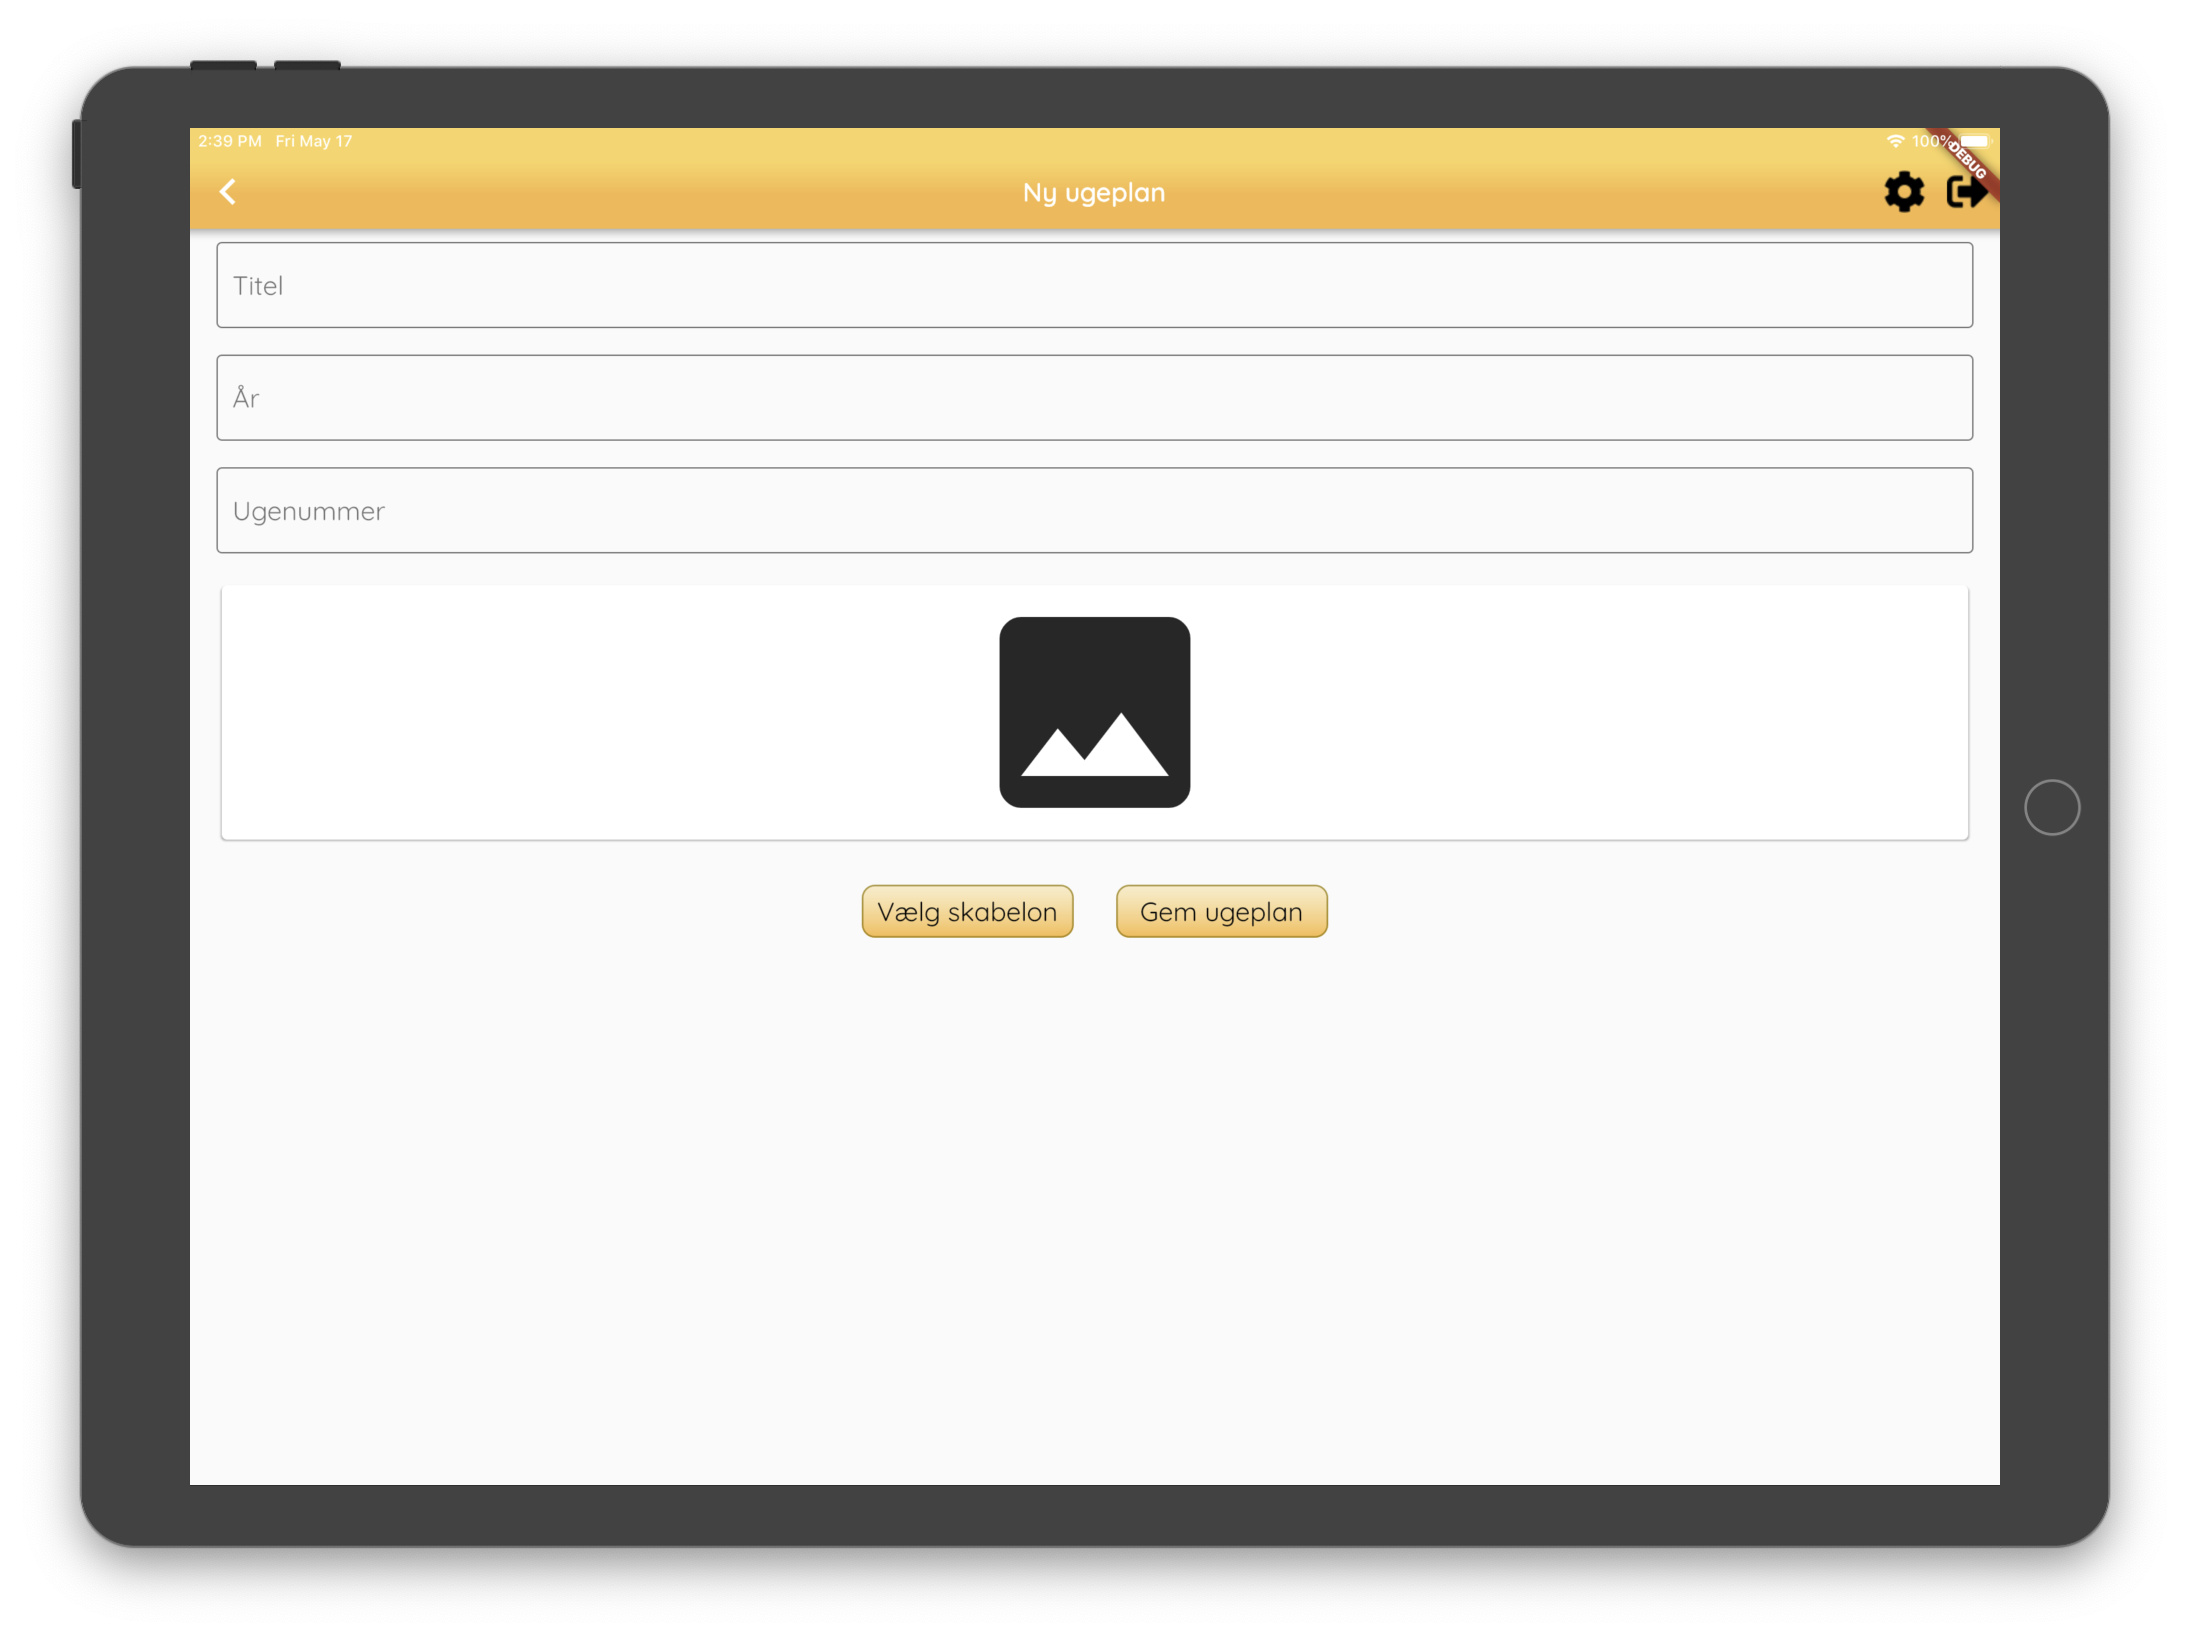
\includegraphics[width=0.7\textwidth]{figures/FinalScreen/addWeekplanScreen.png}
    \end{center}
    \caption{The final new week-plan screen}
    \label{fig:finalAddWeekplanSelector}
\end{figure}

In \autoref{fig:finalAddWeekplanSelector}, which shows the new week-plan screen, we can enter a title, year, week number and picture, and make a new week-plan. If we tab the picture field, we will be redirected to the pictogram search screen, where we can choose a picture for the week-plan.

\subsection{Weekplan Screen}

The week-plan screen has three modes, \gls{guardian} mode, edit mode, and \gls{citizen} mode, shown in \autoref{fig:finalWeekplanMoveActivity}, \autoref{fig:finalWeekplanEditMode}, and in \autoref{fig:finalWeekplanCitizenMode}, respectively.

\begin{figure}[H]
    \begin{center}
        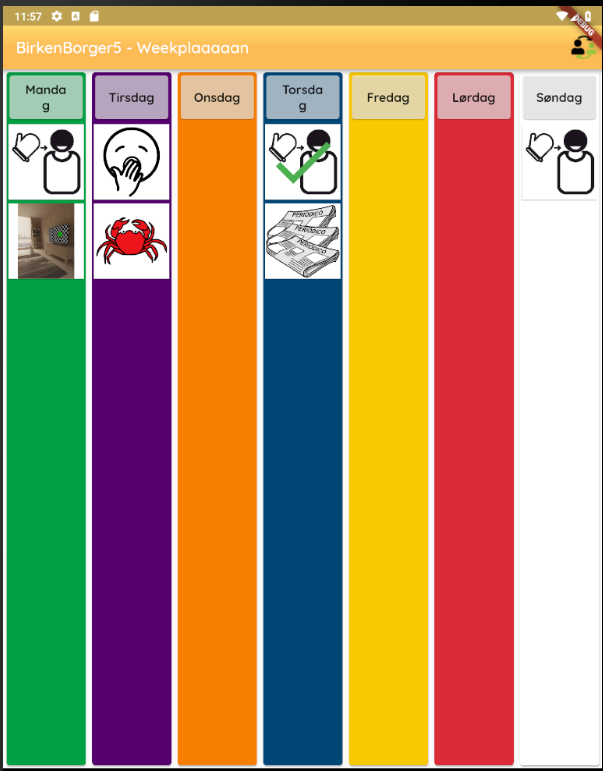
\includegraphics[width=0.7\textwidth]{figures/FinalScreen/weekplanScreenMoveActivity.png}
    \end{center}
    \caption{Move an activity in a weekplan}
    \label{fig:finalWeekplanMoveActivity}
\end{figure}

\begin{figure}[H]
    \begin{center}
        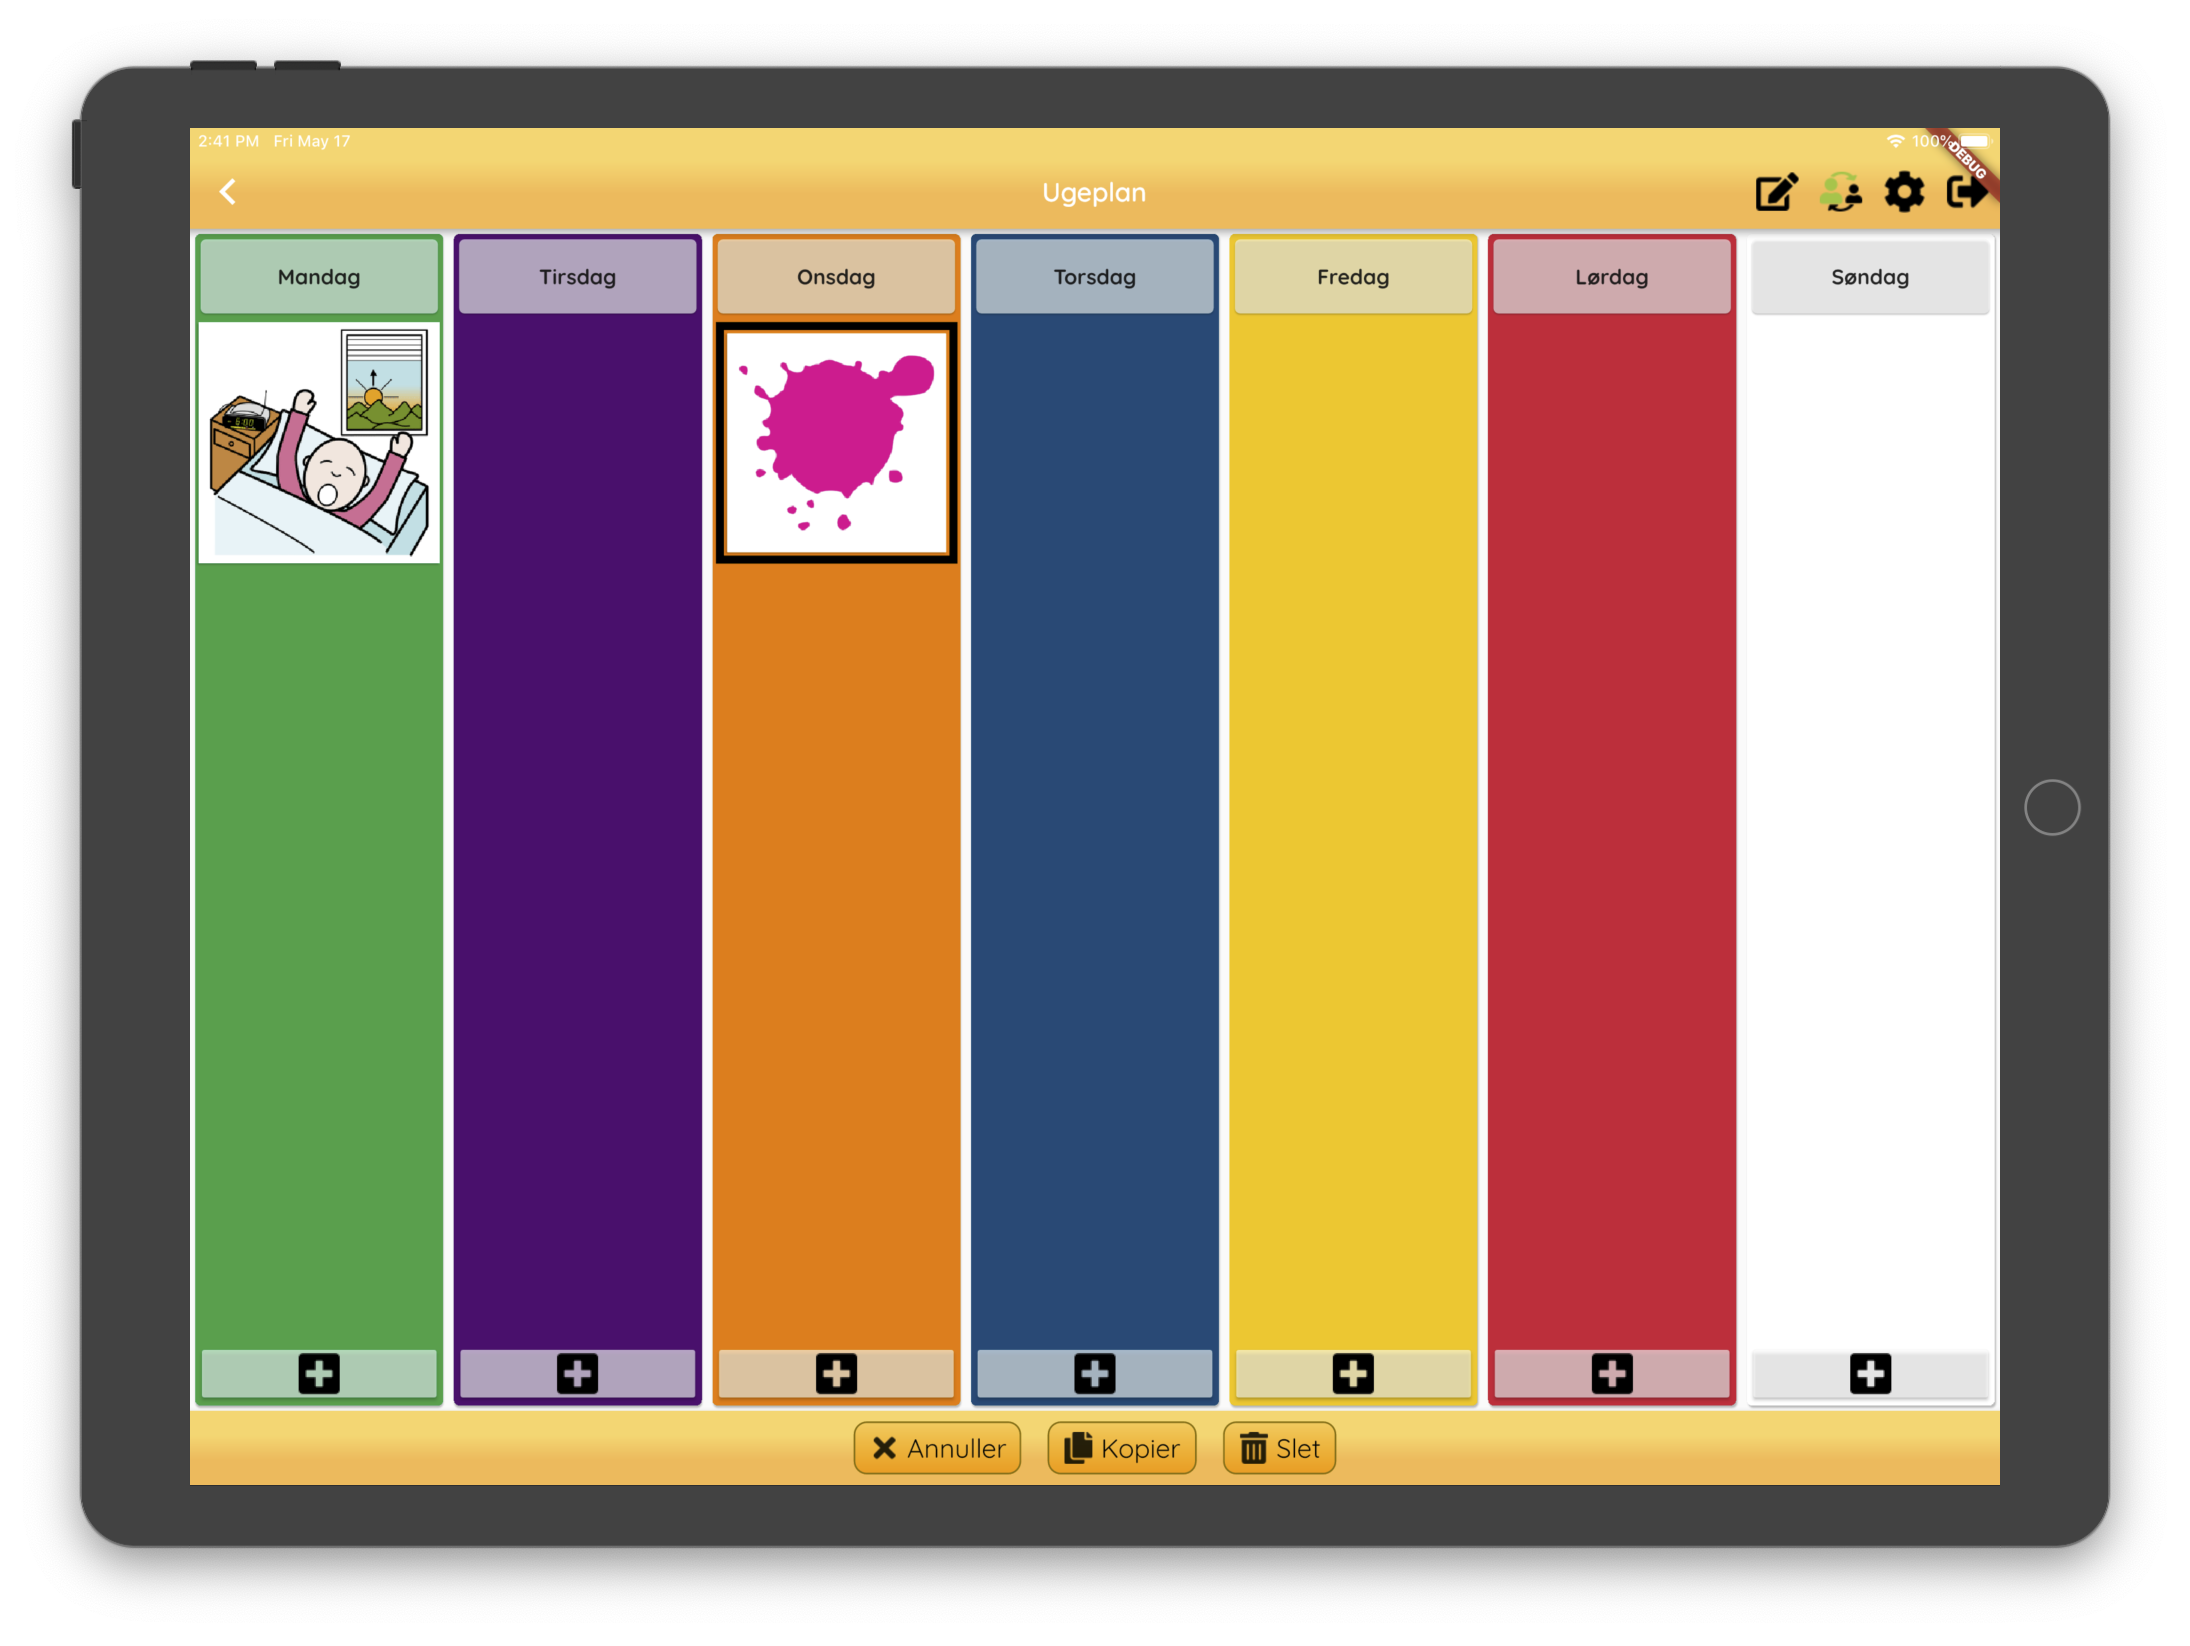
\includegraphics[width=0.7\textwidth]{figures/FinalScreen/editWeekplanScreenMarked.png}
    \end{center}
    \caption{A weekplan screen in edit mode with two activities marked}
    \label{fig:finalWeekplanEditMode}
\end{figure}

\begin{figure}[H]
    \begin{center}
        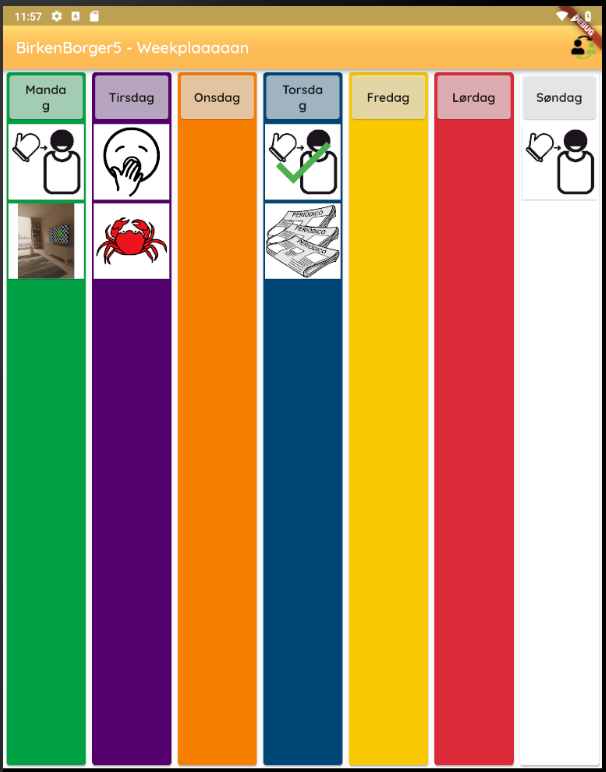
\includegraphics[width=0.7\textwidth]{figures/FinalScreen/weekplanScreenCitizenMode.png}
    \end{center}
    \caption{Final weekplan screen when in citizen mode}
    \label{fig:finalWeekplanCitizenMode}
\end{figure}

When the week-plan screen is in \gls{guardian} mode it is possible to switch to \gls{citizen} or edit mode, enter activities or move activities as in \autoref{fig:finalWeekplanMoveActivity}. When we move an activity we have to hold it a few seconds and then move it to the desired location. It will be placed before the field where we let go.

In edit mode, we can either switch to the other modes, or edit the week-plan. We can mark a variable number of activities, and either delete them or copy them to any number of days. \autoref{fig:finalWeekplanEditMode} shows two selected pictograms. If we want to copy them we click on copy and a popup appears, seen on the left in \autoref{fig:finalCopyEditModeFisk}. The pictograms will then be placed at the end of the chosen days as seen on the right in \autoref{fig:finalCopyEditModeFisk}.

\begin{figure}%
    \centering
    \subfloat[Selecting days]{{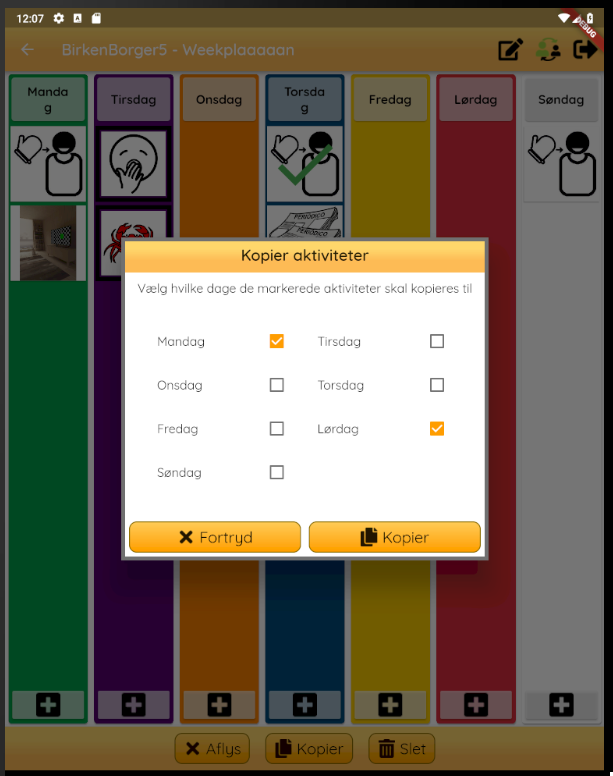
\includegraphics[width=0.45\textwidth]{figures/FinalScreen/editWeekplanScreenCopy.png} }}%
    \quad
    \subfloat[After copying]{{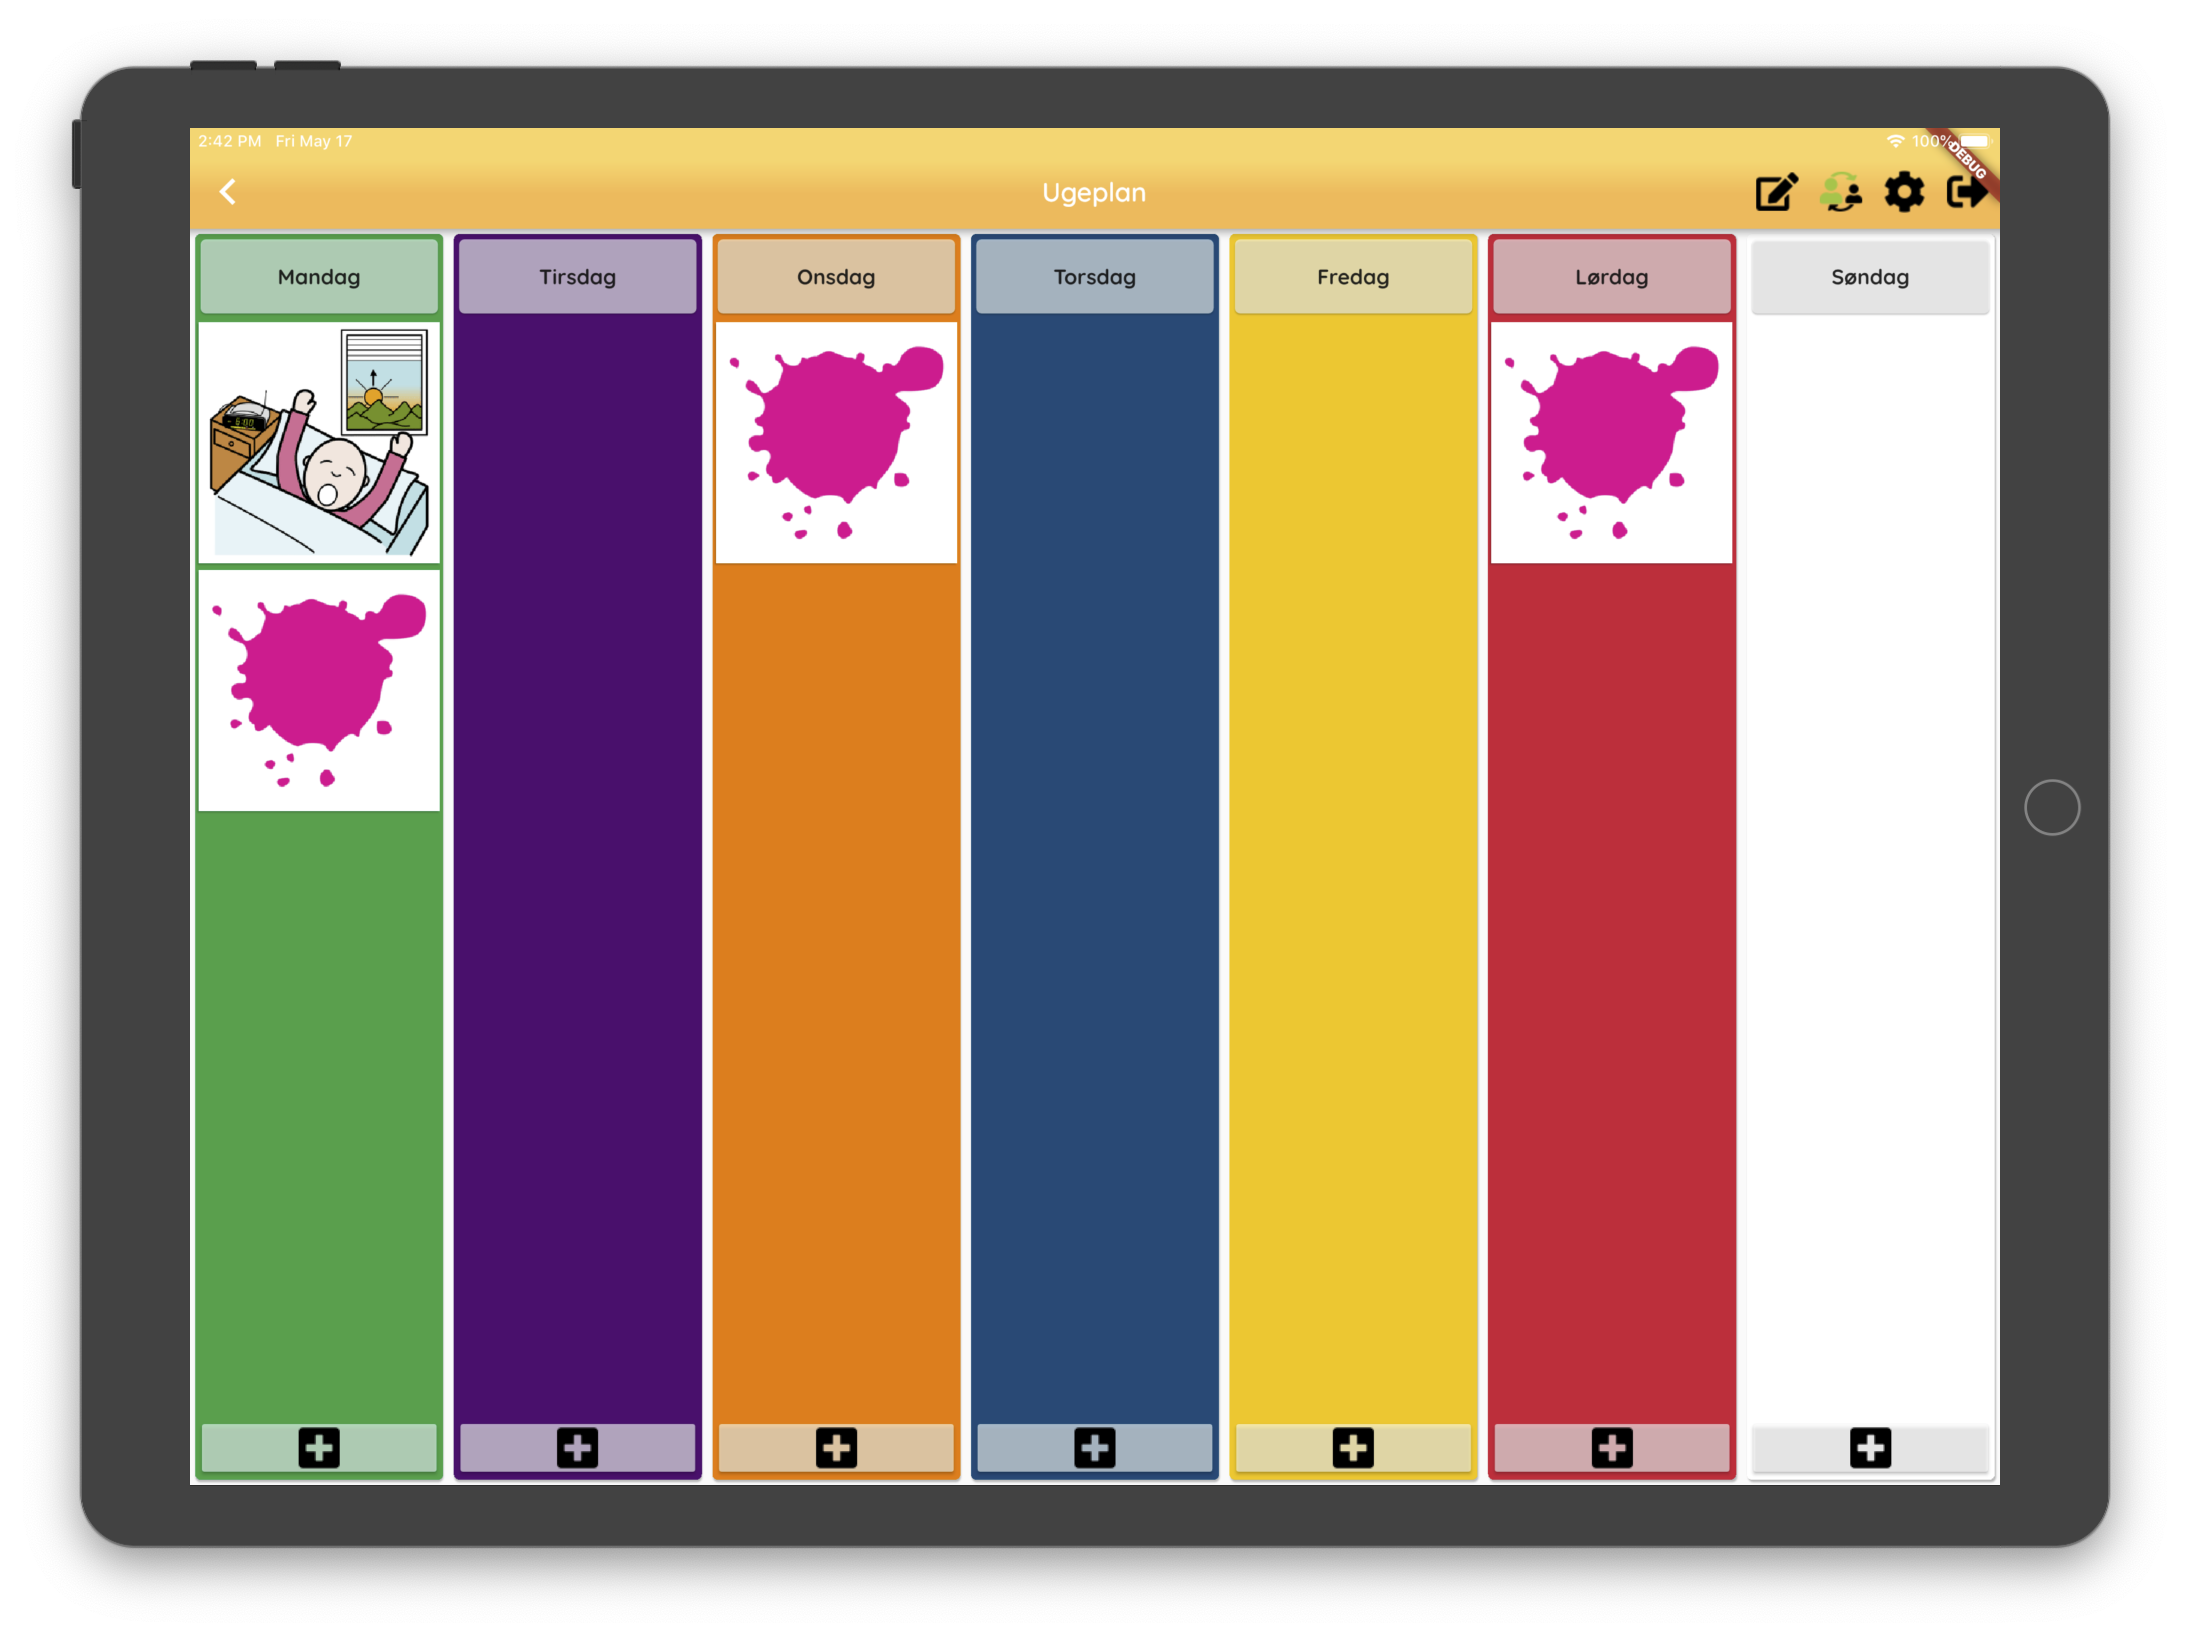
\includegraphics[width=0.45\textwidth]{figures/FinalScreen/editWeekplanScreenAfterCopy.png} }}%
    \caption{Shows the copying ability of the edit mode}%
    \label{fig:finalCopyEditModeFisk}%
\end{figure}

In \gls{citizen} mode, there are fewer functionalities. The \gls{citizen} cannot go back to the select screen, log out or edit in any way. The only things a \gls{citizen} can do is open a show activity screen or change to \gls{guardian}. When a user tries to switch from citizen to \gls{guardian} mode, they have to enter a password, while they only have to confirm the other way round.

\subsection{Pictogram Search Screen}

\begin{figure}[H]
    \begin{center}
        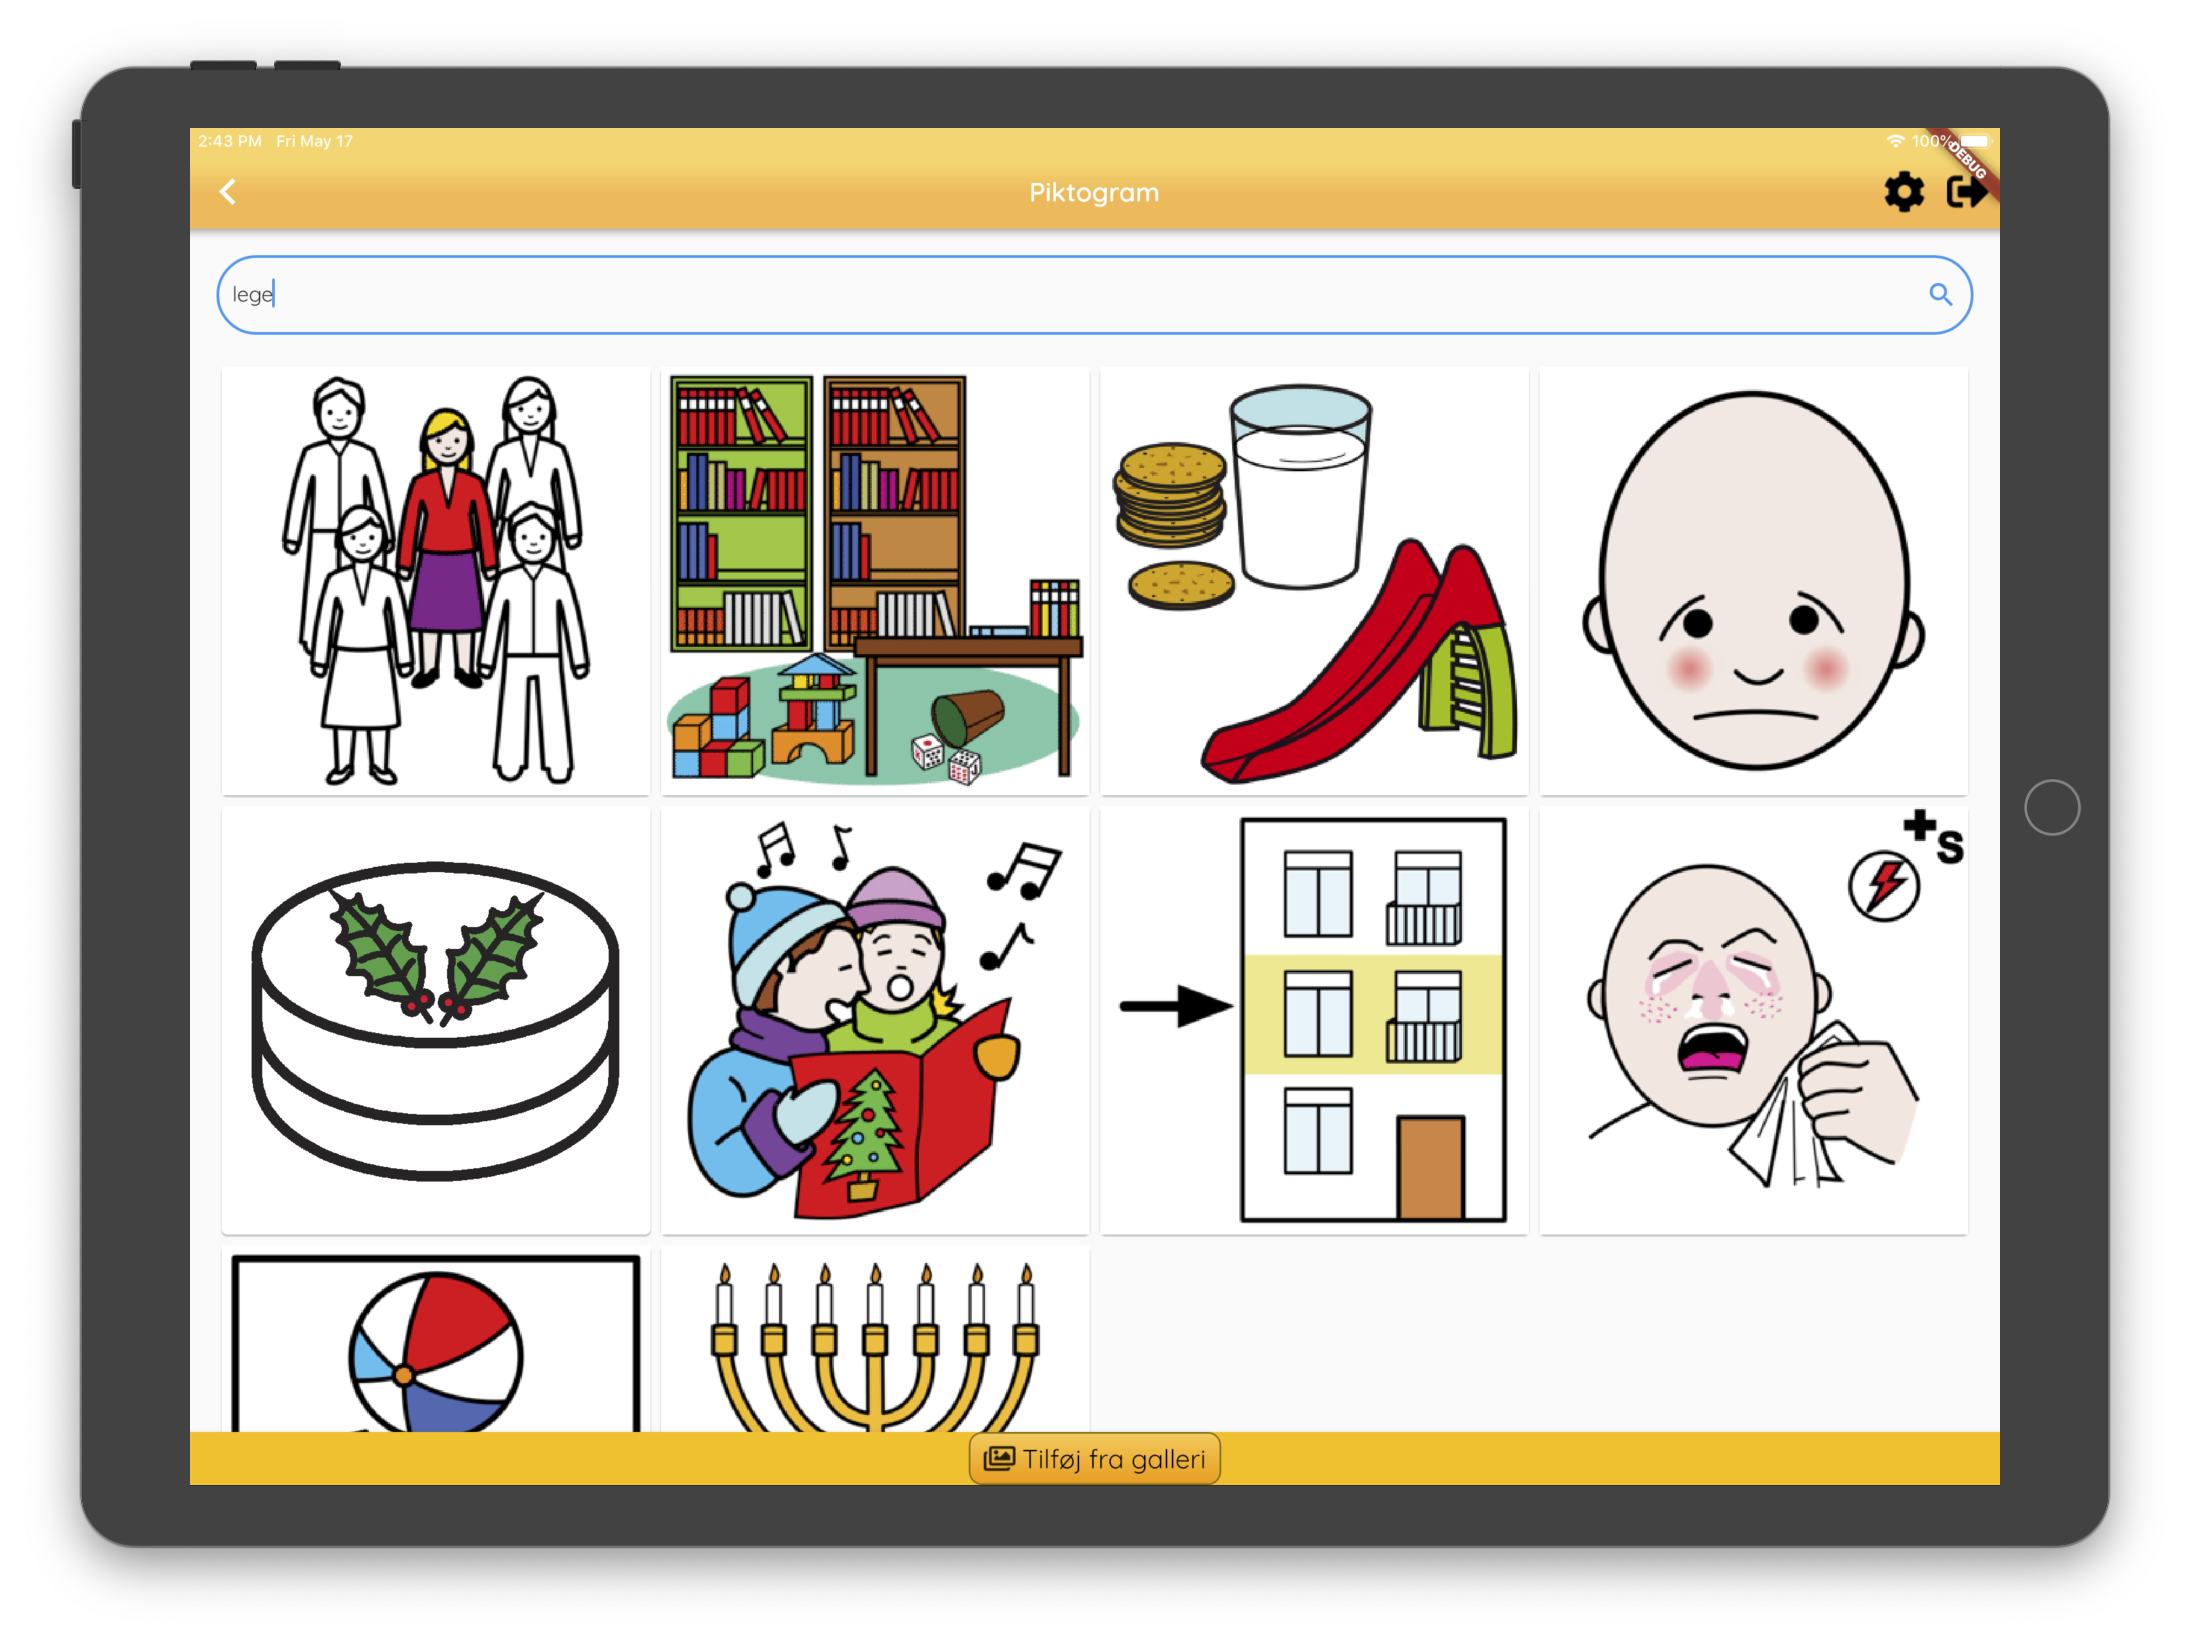
\includegraphics[width=0.7\textwidth]{figures/FinalScreen/addPictogramScreen.png}
    \end{center}
    \caption{The final pictogram search screen}
    \label{fig:finalPictogramSeach}
\end{figure}

The pictogram search screen, as seen in \autoref{fig:finalPictogramSeach},  can search for pictures from the backend. When we enter text in the text field, the screen shows ten pictures with a name that contains the text. Clicking the button at the bottom of the screen will show the upload pictogram screen, where it is possible to upload an image from the device storage as a pictogram.

\subsection{Show activity screen}

The show activity screen looks different if the app is in \gls{citizen} mode compared to \gls{guardian} mode.

\begin{figure}%
    \centering
    \subfloat[Without Timer]{{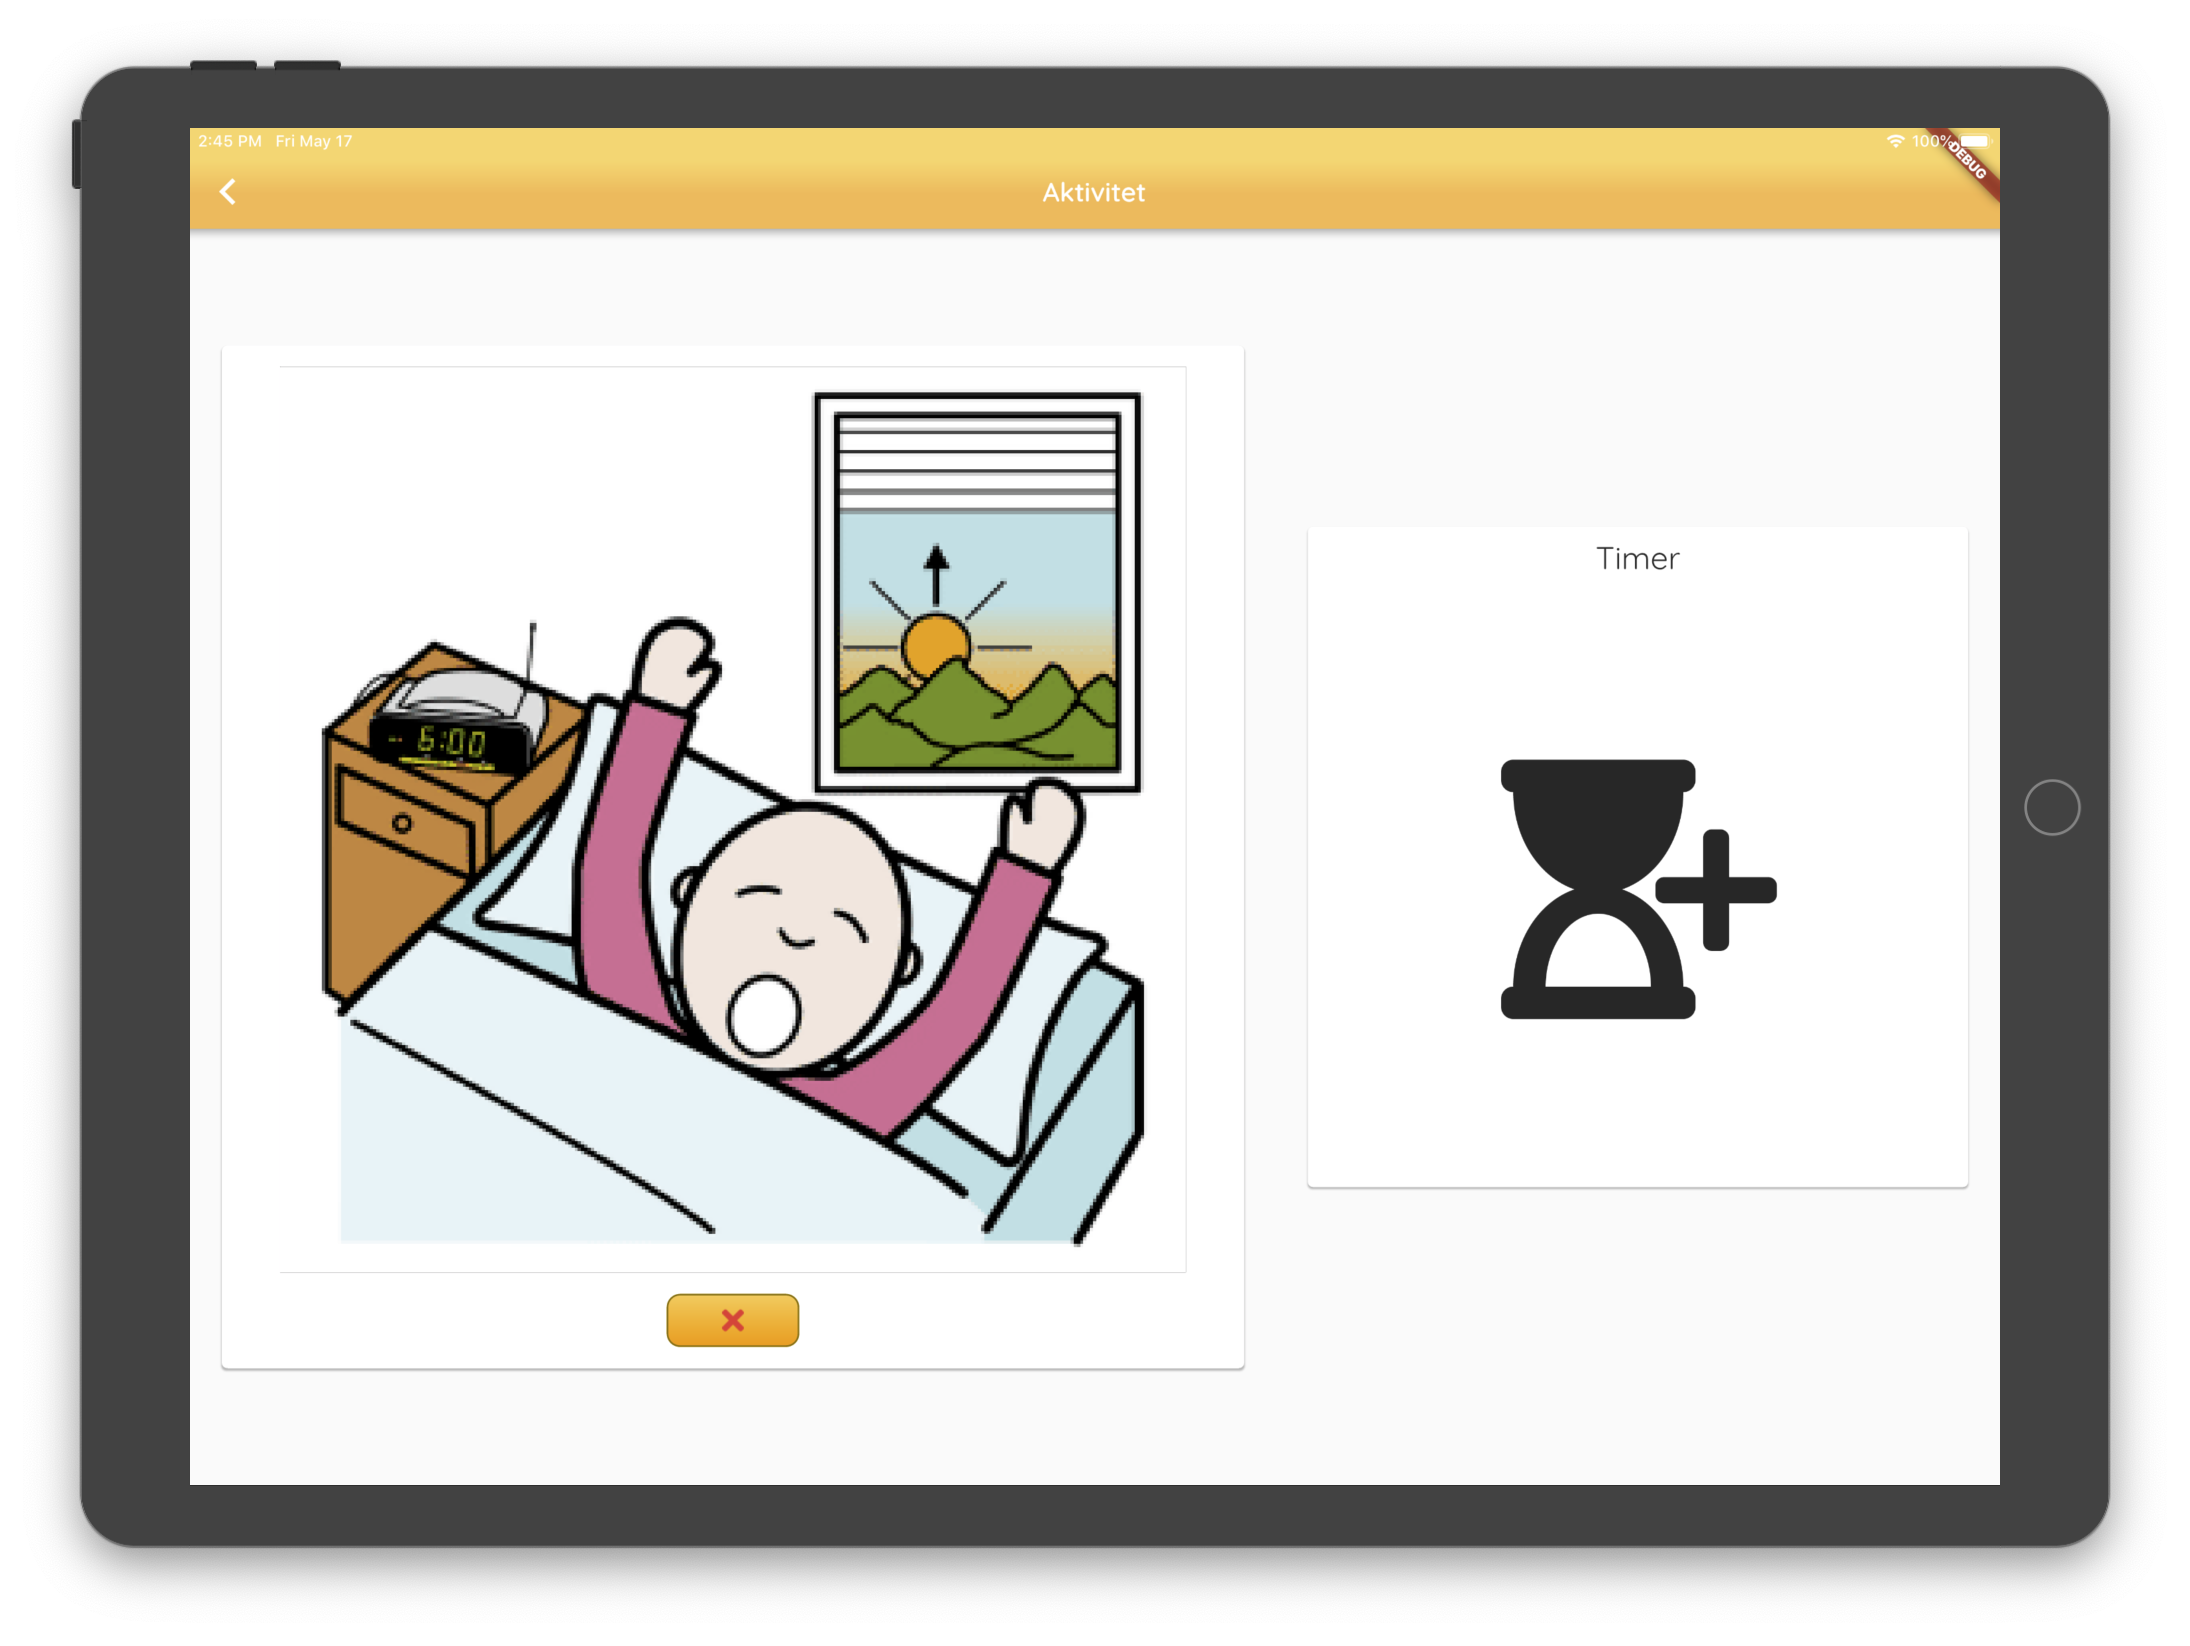
\includegraphics[width=0.45\textwidth]{figures/FinalScreen/showActivityGuardian.png} }}%
    \quad
    \subfloat[With Timer]{{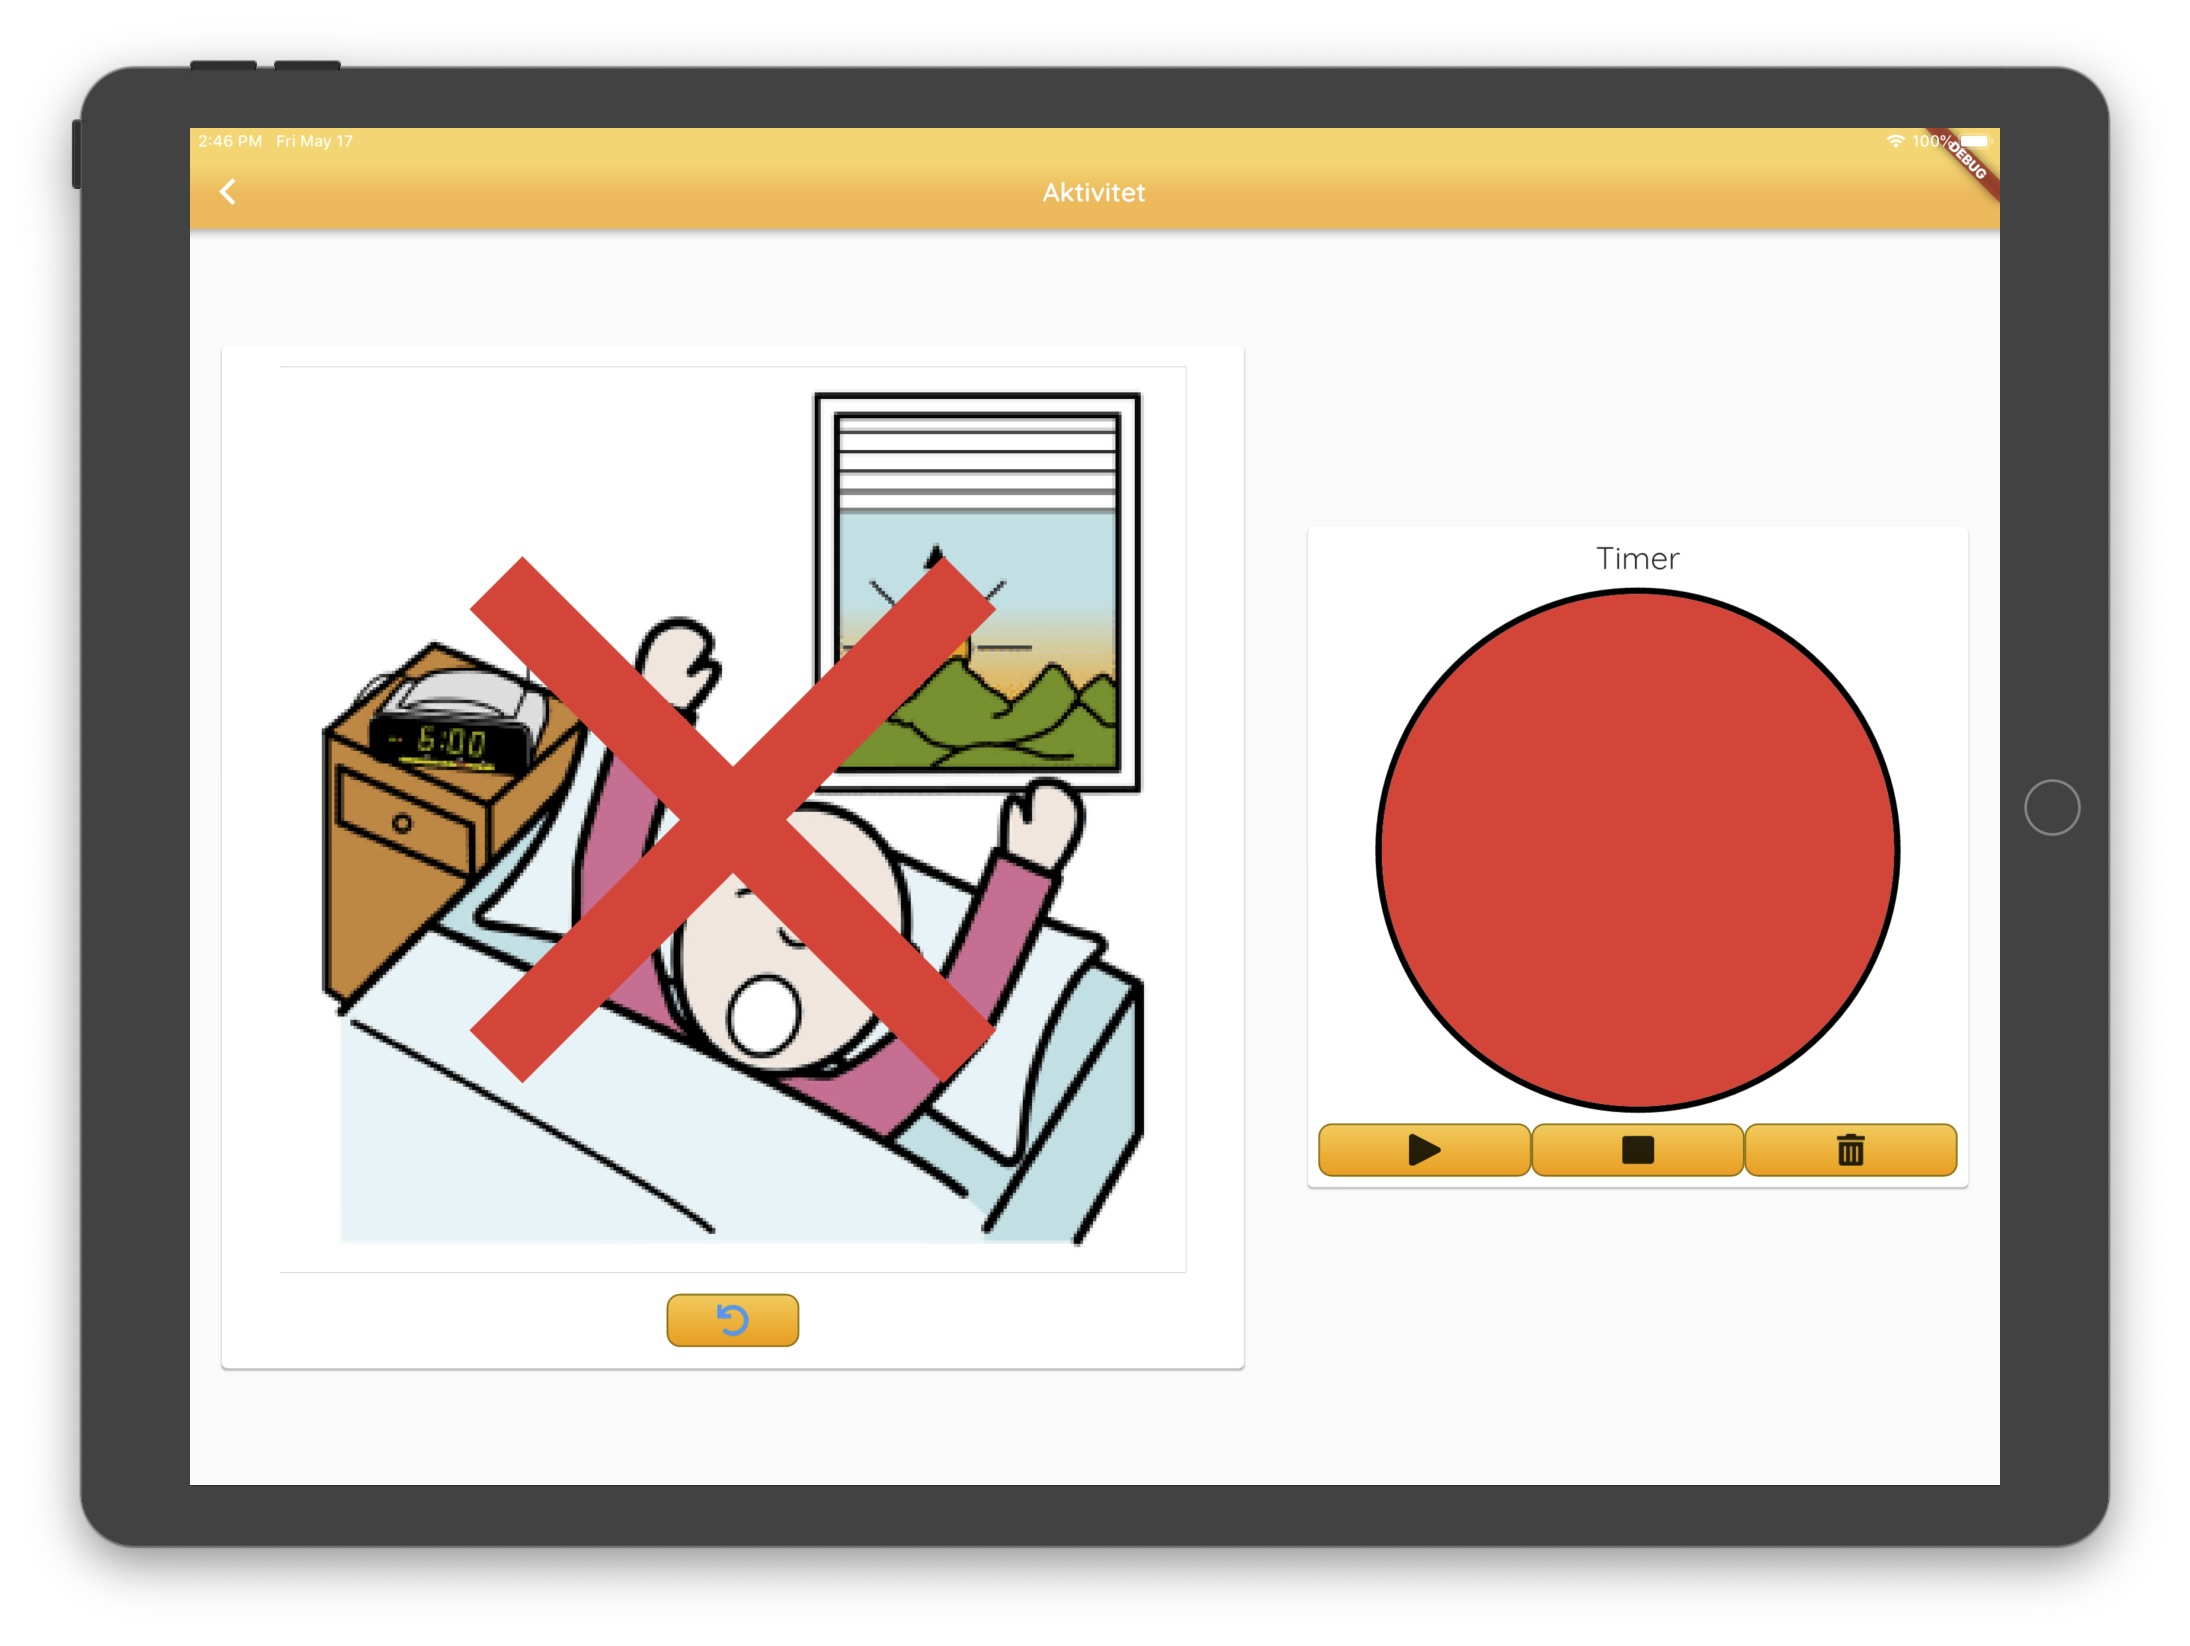
\includegraphics[width=0.45\textwidth]{figures/FinalScreen/showActivityGuardianCanled.png} }}%
    \caption{The final activity screen in \gls{guardian} mode}%
    \label{fig:finalShowActivityGuardianModeFisk}%
\end{figure}

\begin{figure}[H]
    \begin{center}
        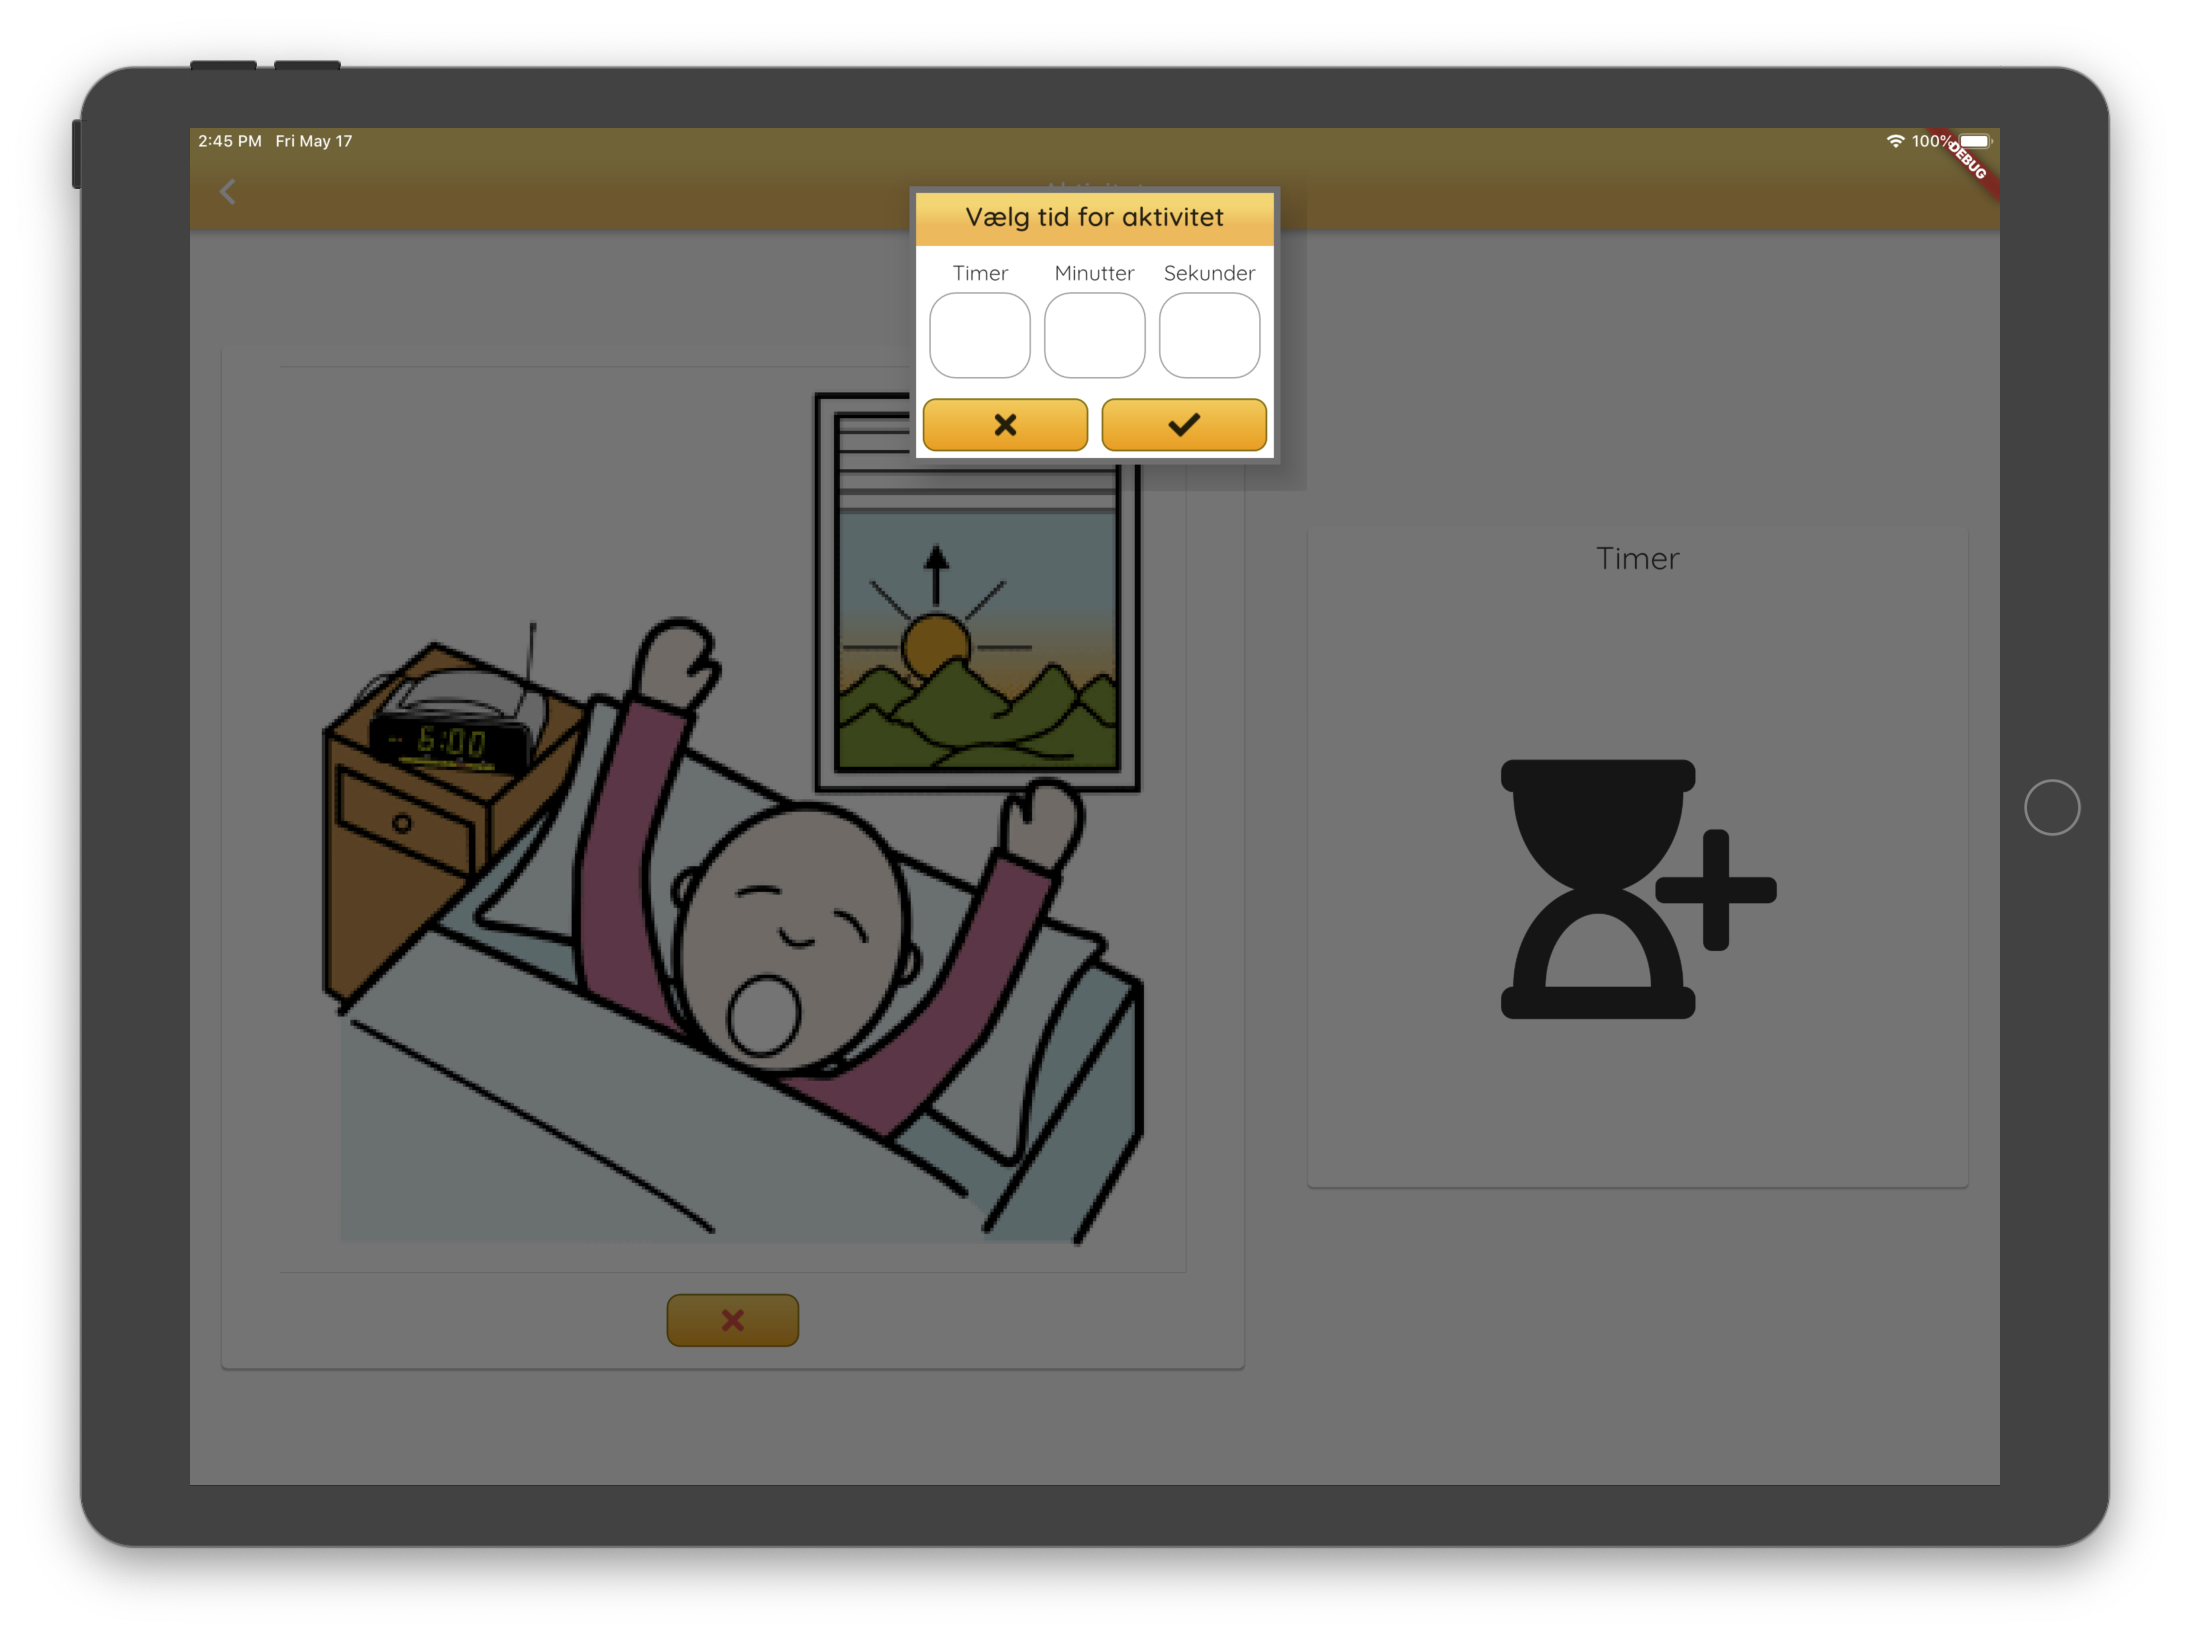
\includegraphics[width=0.7\textwidth]{figures/FinalScreen/showActivityGuardianSetTimer.png}
    \end{center}
    \caption{Set time for activity timer}
    \label{fig:finalShowActivityGuardianSetTimer}
\end{figure}

\begin{figure}%
    \centering
    \subfloat[Without Timer]{{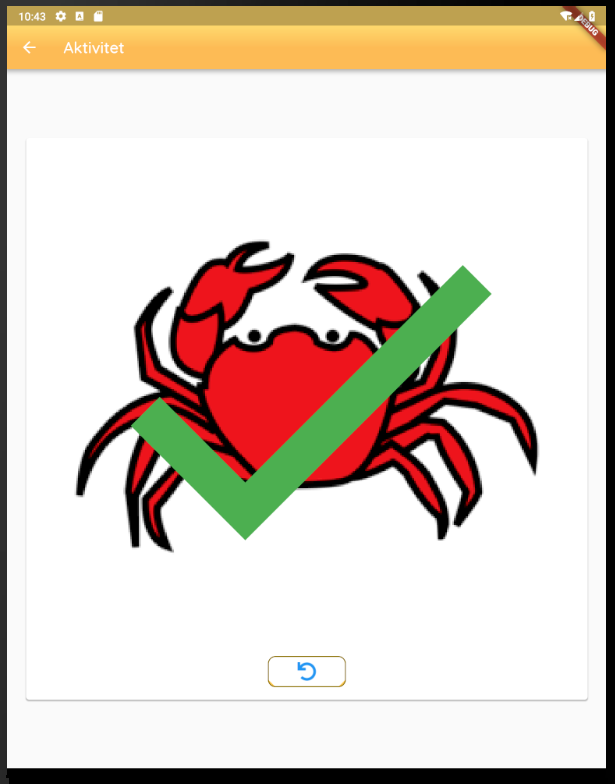
\includegraphics[width=0.45\textwidth]{figures/FinalScreen/showActivityCitizenWithout.png} }}%
    \quad
    \subfloat[With Timer]{{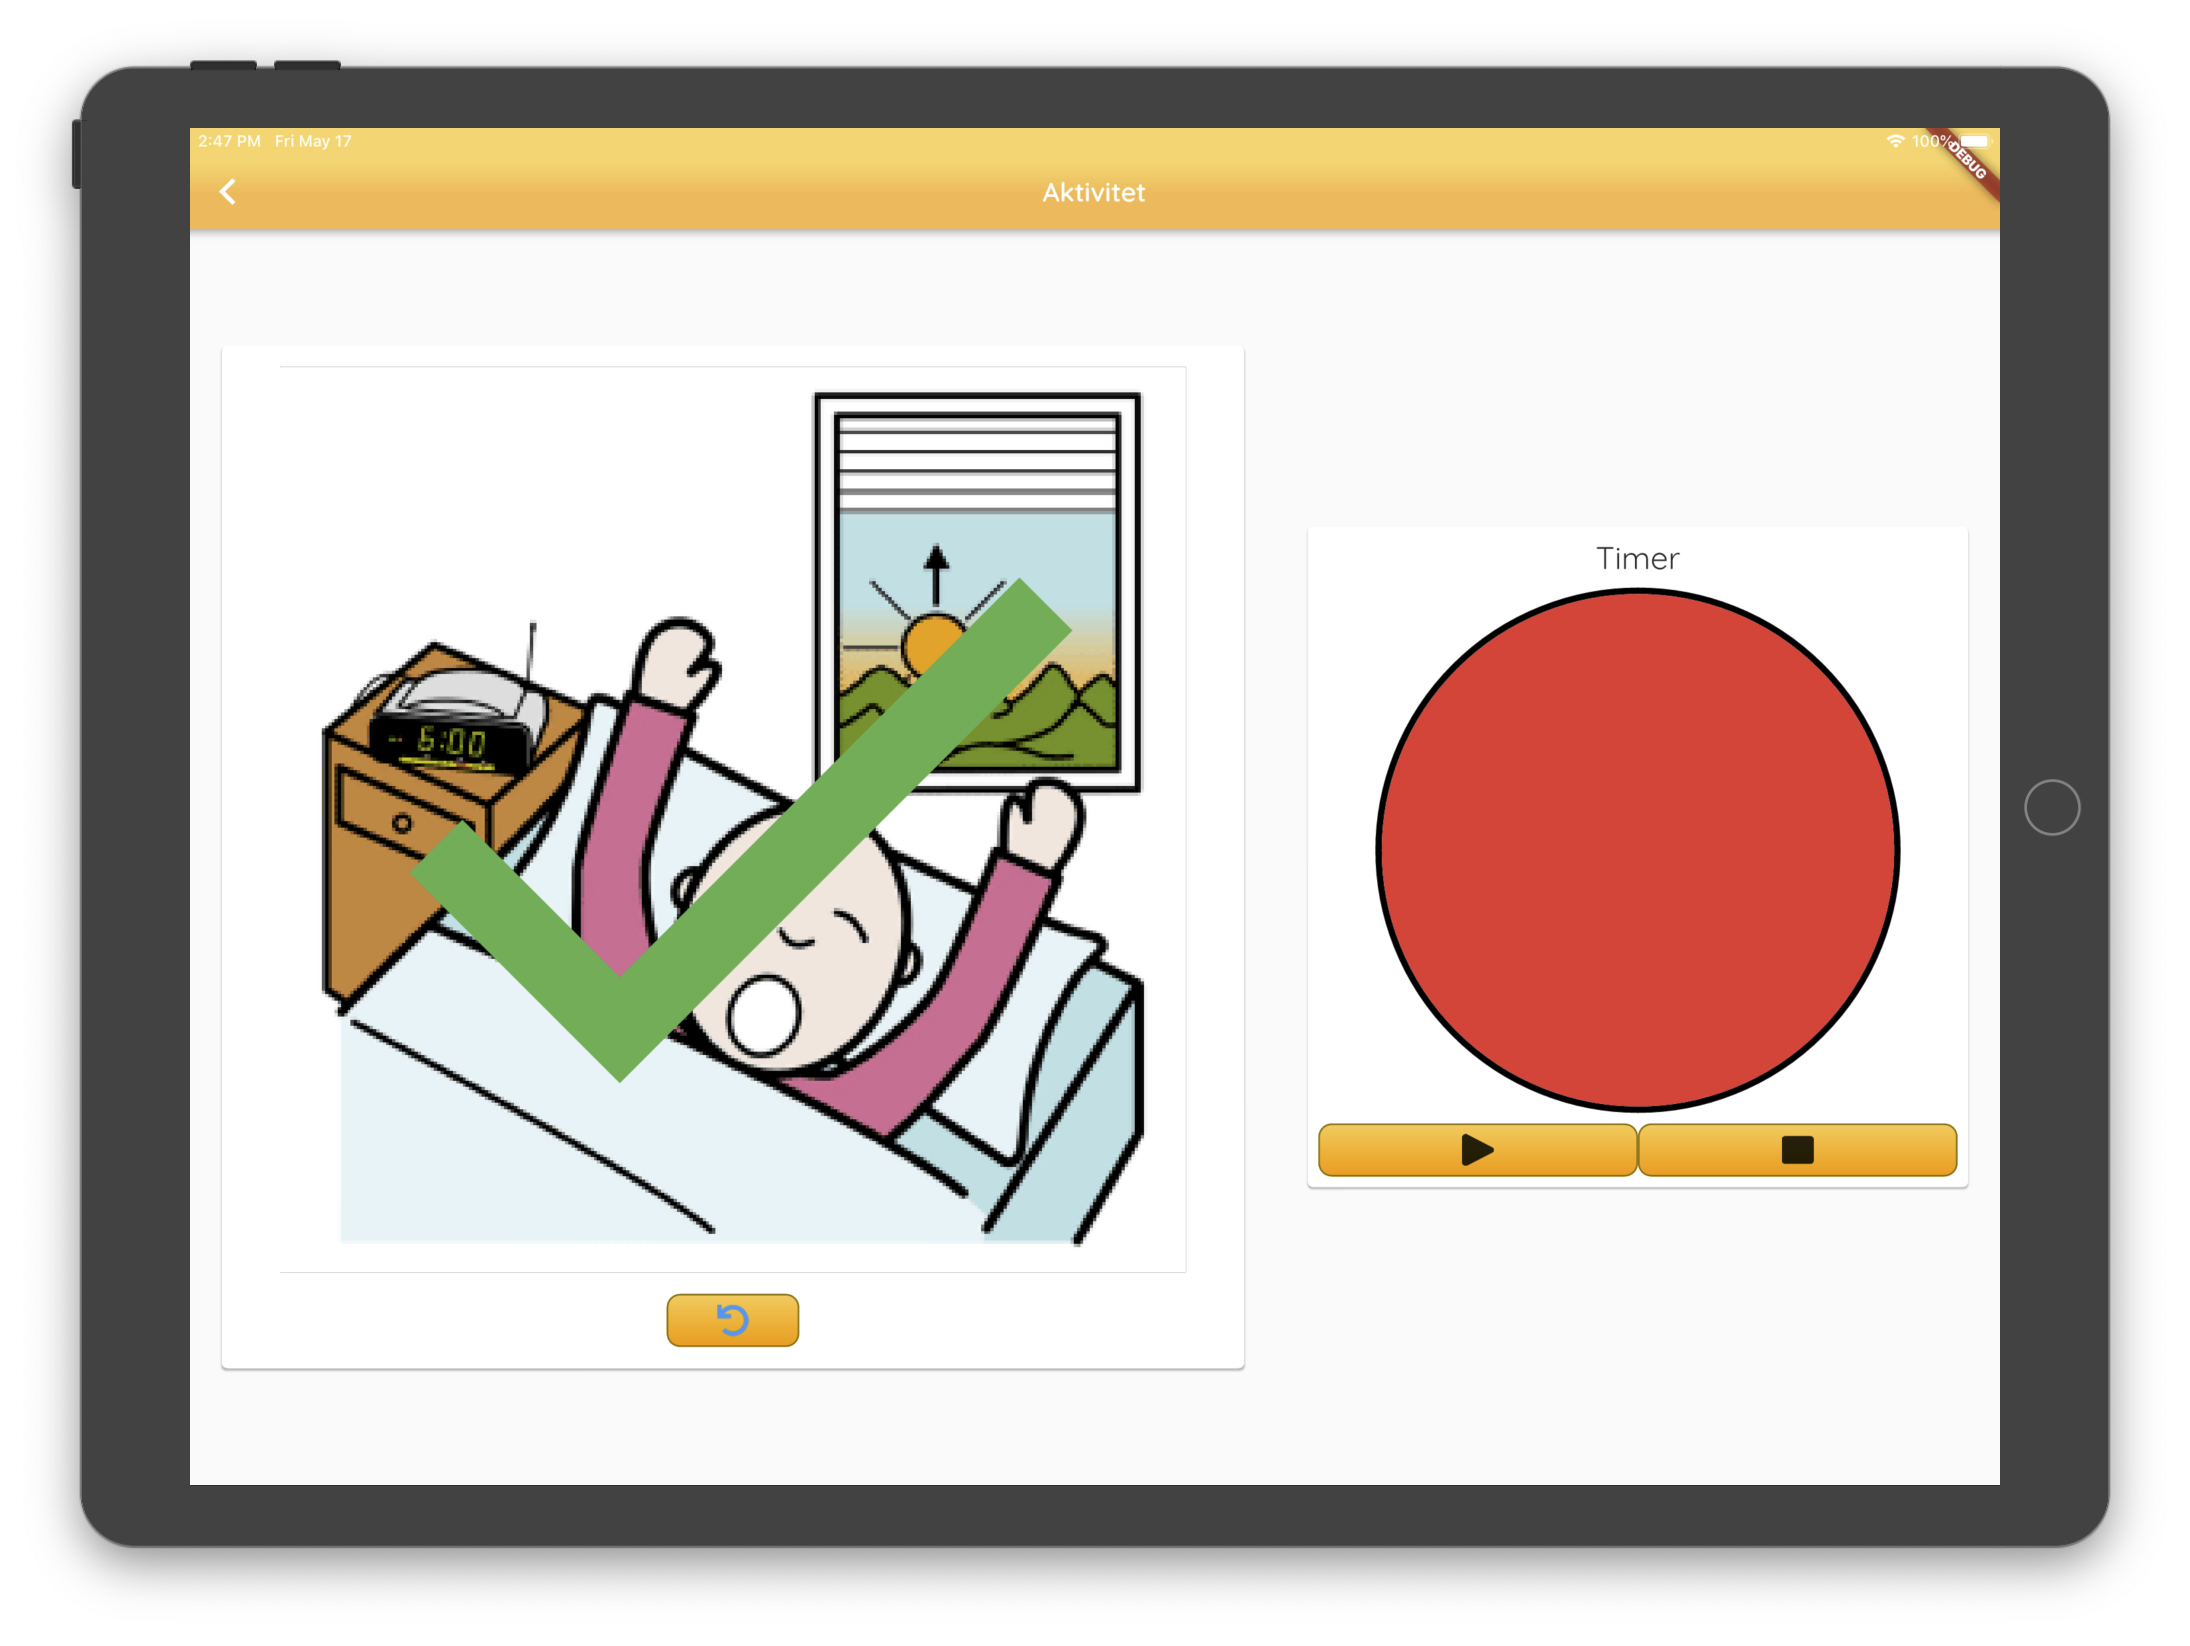
\includegraphics[width=0.45\textwidth]{figures/FinalScreen/showActivityCitizenWithTimer.png} }}%
    \caption{The final activity screen in \gls{citizen} mode}%
    \label{fig:finalShowCitizenActivityModeFisk}%
\end{figure}

In \gls{guardian} mode, an activity can be canceled or uncanceled, or a timer can be set. \autoref{fig:finalShowActivityGuardianModeFisk} shows the screen before and after a timer is set. When setting a timer, the duration should be entered in the fields shown in \autoref{fig:finalShowActivityGuardianSetTimer}, and a timer appears. The timer can be started, paused, stopped, or discarded.

The show activity in citizen mode can be seen in \autoref{fig:finalShowCitizenActivityModeFisk}, where an activity can be marked as done or undone. \Glspl{citizen} can only start, stop, and pause timers.

\subsection{Upload image from phone screen}

The Upload image from phone screen is shown in \autoref{fig:finalUploadPicture}.

\begin{figure}[H]
    \begin{center}
        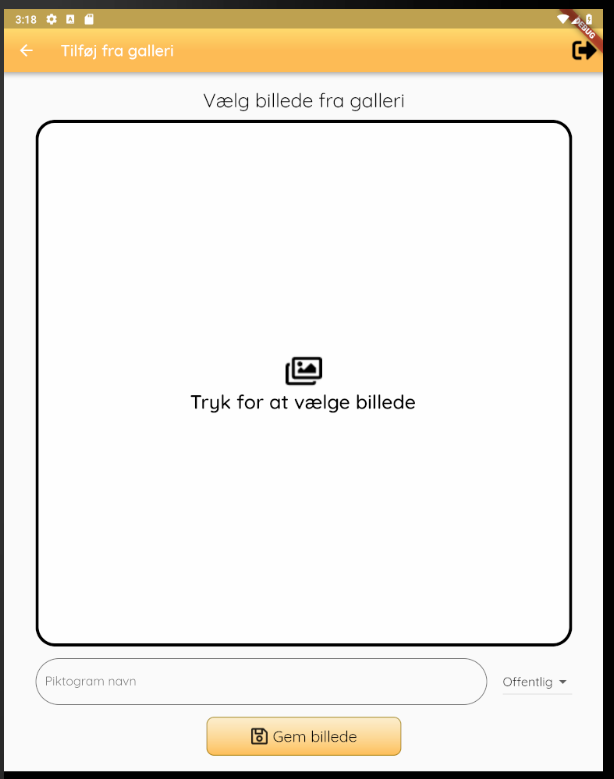
\includegraphics[width=0.7\textwidth]{figures/FinalScreen/addPictogramFromGalleryScreen.png}
    \end{center}
    \caption{The Upload picture from phone screen.}
    \label{fig:finalUploadPicture}
\end{figure}

When the big box is pressed, the phone gallery opens and a picture can be chosen. Before the picture is saved, a pictogram name has to be added in the text box. The option of public or private save is available. The pictogram is added as if it was chosen in the Choose pictogram screen, and saved in the database.

These are the main features and functionalities of the Weekplanner application.